\section{Fast Transfer via Trajectory Decomposition}\label{sec:fast-transfer}

Section~\ref{sec:useful-transfer} demonstrates that without further assumptions, the existence of a scale-independent limit of optimal HP (i.e., \textit{weak transfer}) does not entail that transfer is more computationally efficient than direct tuning. At a high-level, for useful transfer to occur in practical neural network optimization settings, the optimal HPs should depend on some statistics of the training trajectory that converge faster than statistics tied to the performance metric of interest. 
In this section, we explicitly extract the fast-converging statistics from the trajectory and connect them to the optimal HPs. 
To do so, we will leverage prior intuition on the \textit{low-dimensionality} of optimization trajectories (see Section \ref{sec:related_work}): intuitively speaking, we may expect the movement in a small number of HP-sensitive directions to significantly contribute to the loss decrease and approximately determine the optimal HP. If the associated low-dimensional statistics converge sufficiently fast, then the optimal HP also becomes stable across scale. For instance, it is plausible that the loss depends on all eigenvalues of the Hessian, whereas the learning rate is decided by the top components alone (which may converge faster with scale). In the ensuing subsection, we introduce a novel layer-wise spectral decomposition to identify the low-dimensional structure that informs the HP selection.


\subsection{\texorpdfstring{Top-$k$ Loss Decomposition}{Top-k Loss Decomposition}}\label{sec:topk_decomposition}


Let us consider an optimization trajectory $\traj = (\bw_0, \ldots, \bw_T)$ of a neural network. Define the one-step loss change $\delta \loss(\bw_t) := \loss(\bw_{t+1}) - \loss(\bw_t)$, so that the overall loss change is the sum
\[
\Delta \loss(\traj) := \loss(\bw_T) - \loss(\bw_0) = \sum\limits_{t=0}^{T-1} \delta \loss(\bw_t).
\]
Let $\bg_t := \grad \loss(\bw_t)$ and $\delta \bw_t := \bw_{t+1} - \bw_t$. Let us define $\delta \phi(\bw_t) := \inner{\bg_t}{\delta \bw_t}$ to be the linearization of $\delta \loss(\bw_t)$. Under appropriate smoothness conditions on the trajectory,
\begin{equation}\label{eq:linear_defs}
    \delta \phi(\bw_t) \approx \delta \loss(\bw_t)
\text{ ~~and~~ } \phi(\traj) := \sum\limits_{t=0}^{T-1} \delta \phi(\bw_t) \approx \Delta \loss(\traj).
\end{equation}
To ensure that such smoothness conditions hold and $\phi(\traj)$ is a useful proxy for $\Delta \loss(\traj)$, we take $\traj$ to be an \textit{exponential moving average} (EMA) of the base optimization trajectory to remove oscillatory behavior. Empirically, on realistic problems, we obtain excellent agreement between $\phi(\traj)$ and $\Delta \loss(\traj)$ for EMA trajectories which perform at least as well as the corresponding base trajectories (see Fig.\ \ref{fig:ema_iterate_lin}). 
We believe that this approach can be used more broadly in the empirical analysis of neural network optimization since it allows us to accurately approximate an optimization trajectory as the discretization of a continuous-time flow. 


The utility of considering the linearization $\phi(\traj)$ in our setting is that we can decompose $\delta \phi(\bw_t)$ based on the structure of $(\bg_t, \delta \bw_t)$ and recover a resulting decomposition of $\phi(\traj)$. Let us consider a fixed time index $t$. If $\bw = (\bW^{(1)}, \ldots, \bW^{(L)})$ are the model parameters with corresponding gradients $\bg = (\bG^{(1)}, \ldots, \bG^{(L)})$ such that $\bW^{(\ell)}$ and $\bG^{(\ell)}$ are tensors of the same shape, then 
\[
    \inner{\bg}{\delta \bw} = \sum\limits_{\ell \in [L]} \inner{\bG^{(\ell)}}{\delta \bW^{(\ell)}}.
\]
Consider a single summand coming from $\bW \in \R^{m \times n}$ with corresponding gradient $\bG \in \R^{m \times n}$. To
isolate the dominant directions of descent, we analyze the alignment between the gradient and the update via the \emph{alignment matrix} which is the symmetrized product:
\begin{equation}\label{eq:alignmat}
    \sym(\bG, \delta \bW) := \textstyle\frac{1}{2}(\bG^\top \cdot \delta \bW + \delta \bW^\top \cdot \bG).
\end{equation}
If $\sym(\bG, \delta \bW)$ has eigenvalues $\lambda_1, \ldots, \lambda_n$ such that $|\lambda_1| \geq \cdots \geq |\lambda_n|$, then the loss change $\delta \phi(\bW)$ from the update to $\bW$ is the sum of the eigenvalues, and we define the top-$k$ stepwise linear loss change $\delta \phi^k(\bW)$ to be the sum of the first $k$ eigenvalues.
\begin{equation}\label{eq:topk-loss-param}
    \delta \phi(\bW) = \sum\limits_{i=1}^n \lambda_i~~ \text{ and }~~ \delta \phi^k(\bW) := \sum\limits_{i = 1}^k \lambda_i.
\end{equation}
Eq.\ \eqref{eq:topk-loss-param} captures an intuitive notion of the loss change in the top-$k$ directions of maximum change in loss. If the update $\delta \bW$ is aligned with the gradient, i.e., $\bG \propto  \delta \bW$, then $\delta \phi^k(\bW)$ is the sum of the top-$k$ singular values of $\bG$. We can add the stepwise changes over time and parameters\footnote{We will only decompose matrix parameters and use the full inner-product for vector parameters. \vspace{-2mm}} to compute the top-$k$ loss change, 
\begin{equation}\label{eq:topk-loss}
    \phi^k(\traj) := \sum\limits_{\ell \in [L]} \sum\limits_{t = 0}^{T-1} \delta \phi^k\qty(\bW^{(\ell)}_t). 
\end{equation}

For some parameters we employ a ``row version'' of $\delta \phi^k$ which uses $\sym(\bG^\top, \delta \bW^\top)$ in place of $\sym(\bG, \delta \bW)$. Then the index $k$ can span $[n]$ across all layers so that using the same $k$ for each layer in Eq.\ \eqref{eq:topk-loss} is reasonable.  

\begin{table}[t]
\vspace{-4mm}
    \centering
    \caption{\rev{\small Notation for the linearized trajectory decomposition.}}
    \vspace{-2mm}
    \label{tab:phi_notation}
    \small
    \begin{tabular}{@{}llc@{}}
        \toprule
        \textbf{Symbol} & \textbf{Definition} & \textbf{Ref.} \\
        \midrule
        $\delta \phi(\bw_t)$ & Linearized loss change at step $t$. & \eqref{eq:linear_defs} \\
        $\phi(\traj)$ & Total sum of $\delta \phi(\bw_t)$ over trajectory. & \eqref{eq:linear_defs} \\
        $\delta \phi^k(\bW^{(\ell)}_t)$ & Sum of top-$k$ components in layer $\ell$ at time $t$. & \eqref{eq:topk-loss-param} \\
        $\phi^k(\traj)$ & Sum of top-$k$ components over layers and time. & \eqref{eq:topk-loss} \\
        \midrule
        $\phi_n(\bhp)$ & Loss curve over HPs $\bhp$ for width $n$. & \eqref{eq:decomposition_quantities} \\
        $\hptrunc(\bhp)$ & Truncation function maps HPs $\bhp$ to index in $[n]$. & \eqref{eq:decomposition_quantities} \\
        $\phi_n^\hptrunc(\bhp)$ & HP adaptive top-$\hptrunc$ loss curve $\phi_n^{\hptrunc(\bhp)}(\bhp)$. & \eqref{eq:decomposition_quantities} \\
        \bottomrule
    \end{tabular}
\end{table}


\paragraph{Decomposition-aware HP Transfer.}
We can now make our earlier intuitions in Hypothesis~\ref{box:fast-transfer} more precise using this stepwise decomposition. Assume we fix a training procedure $\algo$ (see Definition \ref{def:hp_transfer}).
Then we can define the width-$n$ trajectory trained with HPs $\bhp$ and scaling $\bhpexp$ to be the trajectory $\traj_n(\bhp, \bhpexp)$ obtained from executing the training procedure $\algo$ with hyperparameters $\scaledhps_n(\bhp, \bhpexp)$. If we consider a fixed scaling $\bhpexp$ and an HP-dependent \emph{truncation function} $\hptrunc$ which outputs an index $\hptrunc(\bhp) \in [n]$ given HPs $\bhp$, we can abbreviate 
\begin{align}\label{eq:decomposition_quantities}
    &\phi_n(\bhp) := \phi(\traj_n(\bhp, \bhpexp)),~  \phi_n^\hptrunc(\bhp) := \phi^{\hptrunc(\bhp)}(\traj_n(\bhp, \bhpexp)) \notag \\
    &\bhp^\star(n) := \argmin_{\bhp} \phi_n(\bhp),~  \bhp_\hptrunc^\star(n) := \argmin_{\bhp} \phi^{\hptrunc(\bhp)}_n(\bhp).
\end{align}
We will refer to $\phi_n^\hptrunc$ as the \textbf{top-$\hptrunc$ loss curve} and $\phi_n^{-\hptrunc} := \phi_n - \phi_n^\hptrunc$ as the \textbf{residual loss curve}. For
convenience, we summarize the notation for our trajectory decomposition in Table \ref{tab:phi_notation}.

Based on this decomposition, we have the following conceptual explanation of fast transfer: if for an appropriately chosen sequence $\hptrunc_n$ the following are simultaneously true for large enough $n$, 
\begin{itemize}[leftmargin=*]
    \item \textbf{Top-$\hptrunc$ strong convexity:} The top-$\hptrunc_n$ losses $\phi_n^{\hptrunc_n}$ and $\phi_\infty^{\hptrunc_n}$ are locally strongly-convex.
    \item \textbf{Top-$\hptrunc$ invariance:} The top-$\hptrunc_n$ loss converges rapidly so $\phi_n^{\hptrunc_n} \approx \phi_\infty^{\hptrunc_n}$ and $\bhp^\star_{\hptrunc_n}(n) \approx \bhp^\star_{\hptrunc_n}(\infty)$.
    \item \textbf{Residual Flatness:} The residuals $\phi_n^{-\hptrunc_n}$ and $\phi_\infty^{-\hptrunc_n}$ are ``flat''; hence $\bhp_{\hptrunc_n}^\star(n) \approx \bhp^\star(n)$ and $\bhp_{\hptrunc_n}^\star(\infty) \approx \bhp^\star(\infty)$.
\end{itemize}
then it follows that $\bhp^\star(n) \approx \bhp^\star(\infty)$, that is, the optimal HP remains stable across widths $n$ (see Appendix \ref{app:fast_transfer} for details). This is precisely the mechanism posited in Hypothesis~\ref{box:fast-transfer}: the top-$\hptrunc_n$ loss optimizer stabilizes quickly as width grows and the residual loss is too flat to significantly shift the optimum of the full loss. Due to the prohibitive computational cost to accurately estimate the scaling of the above quantities in realistic settings, in this work we present \textit{qualitative} evidence that the above conditions hold empirically (hence the notation ``$\approx$''). We leave a more quantitative investigation to future work. 

\paragraph{Selecting the Truncation Function.}
Intuitively, selecting $\hptrunc$ involves a trade-off: we must retain enough components to ensure the top-$\hptrunc$ minimizer approximates the true optimal hyperparameters (requiring larger $k$), while excluding tail components that are width-sensitive (requiring smaller $k$). In Appendix \ref{app:fast_transfer}, we formalize this by defining a quantity $\decompobj_n(\hptrunc)$ which upper bounds the HP gap $b_n$ using quantitative measures of top-$\hptrunc$ invariance and residual flatness. By choosing a truncation $\hptrunc_n^\star$ that minimizes $\decompobj_n(\hptrunc)$, we optimally balance these properties to obtain the tightest upper bound on $b_n$. \rev{Since directly optimizing $\decompobj_n$ is intractable, we instead optimize a proxy objective $\decompobj_{\mathrm{proxy}}(\hptrunc)$ to obtain a truncation $\hat{\hptrunc}(n)$ via Algorithm \ref{alg:compute-hptrunc-all} (Appendix \ref{app:selection_process}). We then validate empirically that $\hat{\hptrunc}(n)$ achieves the desired qualitative properties.}

\subsection{Experimental Results}\label{sec:tf_experiments}
We empirically evaluate the explanation of fast transfer developed in Section~\ref{sec:fast-transfer}. Across all settings, we vary the width $n$ as the scaling dimension and for each width we sweep the peak learning rate using $\mu$P. In Section~\ref{sec:llama_adam} we train Llama-style transformers on WikiText-103 using Adam. We find near-perfect learning-rate transfer, along with top-$k$ invariance and residual flatness as posited in our fast transfer conjecture. In Section~\ref{sec:llama_muon} we repeat the same setup but with Muon and observe that transfer is less stable and top-$k$ invariance is weaker. In Section~\ref{sec:mlp_sgd} we train two-layer MLPs on CIFAR-10 with momentum SGD, and interpret what the top and tail components are capturing by introducing a sample-wise version of the top-$k$ decomposition; we use this refined decomposition to connect the quality of transfer to the ``hardness'' of the samples.  



% \vspace{-1.4mm} 
\subsubsection{Llama with Adam}\label{sec:llama_adam}
We train a Llama-style transformer~\citep{touvron2023llama} using the Adam optimizer~\citep{kingma2014adam} with a warmup-stable-decay (WSD) learning rate schedule~\citep{hu2024minicpm} on WikiText-103~\citep{merity2016pointer} using $\mu$P, and sweep the peak learning rate as shown in Figure~\ref{fig:ema_llama_step_7185}; 
detailed setup can be found in Appendix \ref{app:llama_adam_lr}. 
In Appendix \ref{app:adam_betas}, we further examine the Adam $\beta_1$ and $\beta_2$ hyperparameters in this setting.

\begin{figure}[!htb]
\vspace{-2mm}  
    \centering
    \begin{subfigure}[t]{0.49\linewidth}
        \centering
        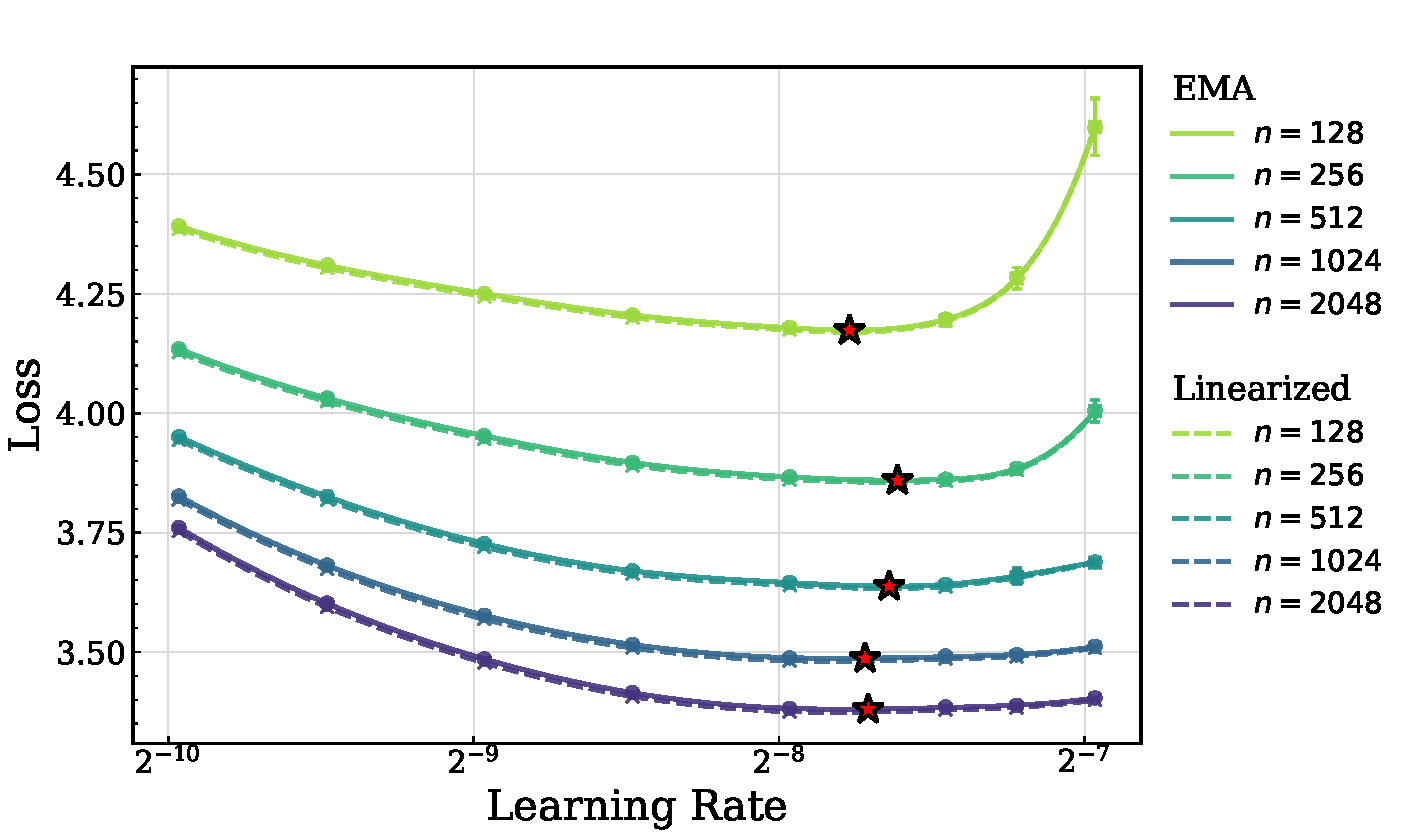
\includegraphics[width=\linewidth]{arxiv_figures/ema_adam_lr_step_7185.pdf}
        % \vspace{-5mm} 
        \caption{EMA loss (solid) and linearized loss (dashed).}
        \label{fig:ema_adam_lr_step_7185}
    \end{subfigure}
    % \hfill
    \hspace{2.5mm}
     \begin{subfigure}[t]{0.4\linewidth}
        \centering
        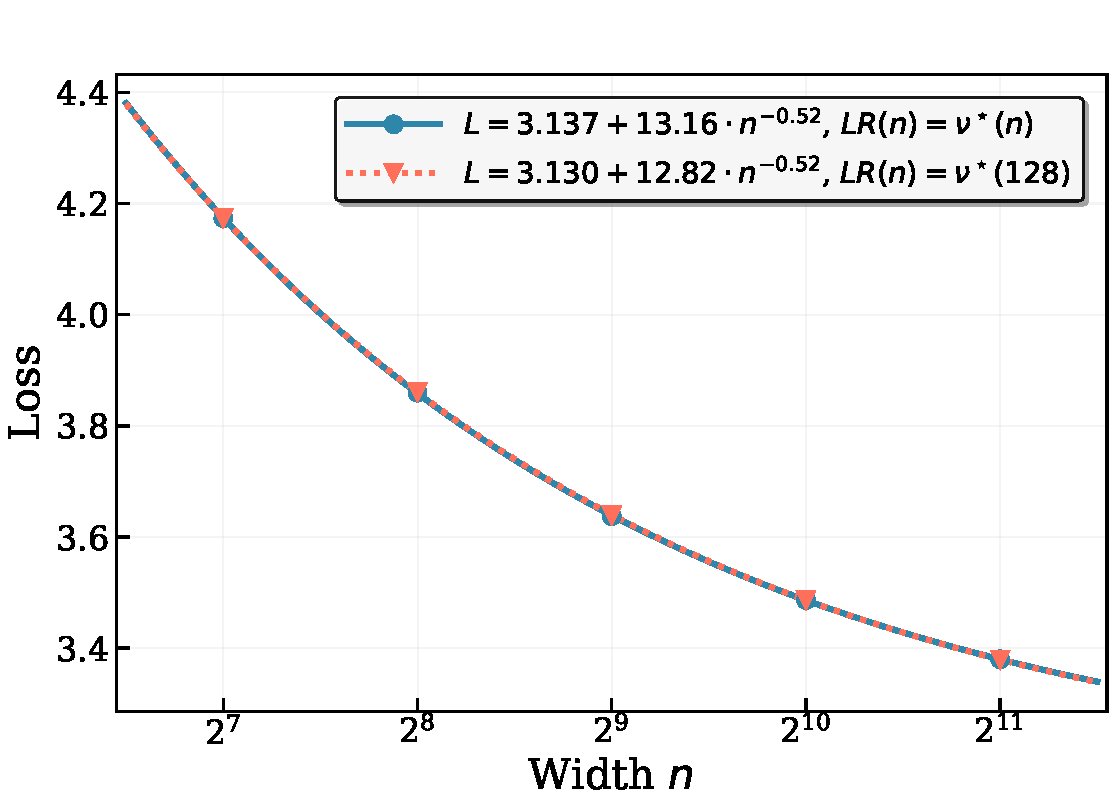
\includegraphics[width=\linewidth]{arxiv_figures/overlay_ema_adam_step_7185.pdf}
        % \vspace{-5mm}
        \caption{Scaling law for the EMA loss.}
        \label{fig:ema_adam_step_7185_scaling_law}
    \end{subfigure}
    % \vspace{-1mm}
    \caption{\small Training a 4-layer Llama transformer with Adam optimizer on WikiText-103. \textbf{Left:} EMA and linearized losses nearly coincide, indicating small linearization error. \textbf{Right:} EMA loss for each width $n$ for two HP choices: 
    the width-dependent optimal learning rate $\hp^\star(n)$ [blue dots] and the  width-$128$ optimal learning rate $\hp^\star(128)$ [orange triangles]. Overlapping curves indicate perfect transfer across widths.
    }
    % \vspace{-1.2mm}
    \label{fig:ema_llama_step_7185}
\end{figure}


\begin{wrapfigure}{r}{0.42\textwidth}  
\vspace{-0.8mm} 
    \centering
    
\includegraphics[width=0.41\textwidth,keepaspectratio]{figures/EMA_ITERATE_LIN_dim=128_lr=0.004_ema=0.9995_seed=0_step_7185.pdf}
    \vspace{-3.6mm}
    \caption{\small Transformer training on WikiText-103. The linearized and EMA losses are identical through training and close to the final iterate loss.}
    \label{fig:ema_iterate_lin}
    \vspace{-7mm}
\end{wrapfigure}


\paragraph{Fast Transfer and Linearization Faithfulness.}  As we can see from Figures \ref{fig:ema_llama_step_7185} and \ref{fig:ema_iterate_lin}, the EMA loss and the linearized loss $\phi$ are nearly indistinguishable, indicating that the EMA trajectory is sufficiently smooth. From Figure \ref{fig:ema_iterate_lin} we see that smoothing does not degrade the final loss. Our setting also clearly exhibits fast transfer since the optimal learning rate is converging rapidly with the width $n$ (see Fig.\ \ref{fig:ema_adam_lr_step_7185}) while the reducible loss improves more slowly, converging at a rate of $n^{-0.52}$ (see Fig.\ \ref{fig:ema_adam_step_7185_scaling_law}). Using the optimal learning rate obtained at width $n = 128$ for larger widths is essentially optimal, as indicated by the overlapping curves in Figure \ref{fig:ema_adam_step_7185_scaling_law}. We now further probe the optimization and scaling dynamics in this fast transfer setting through the lens of our decomposition.

\begin{figure}[b]
\vspace{-3.7mm} 
    \centering
    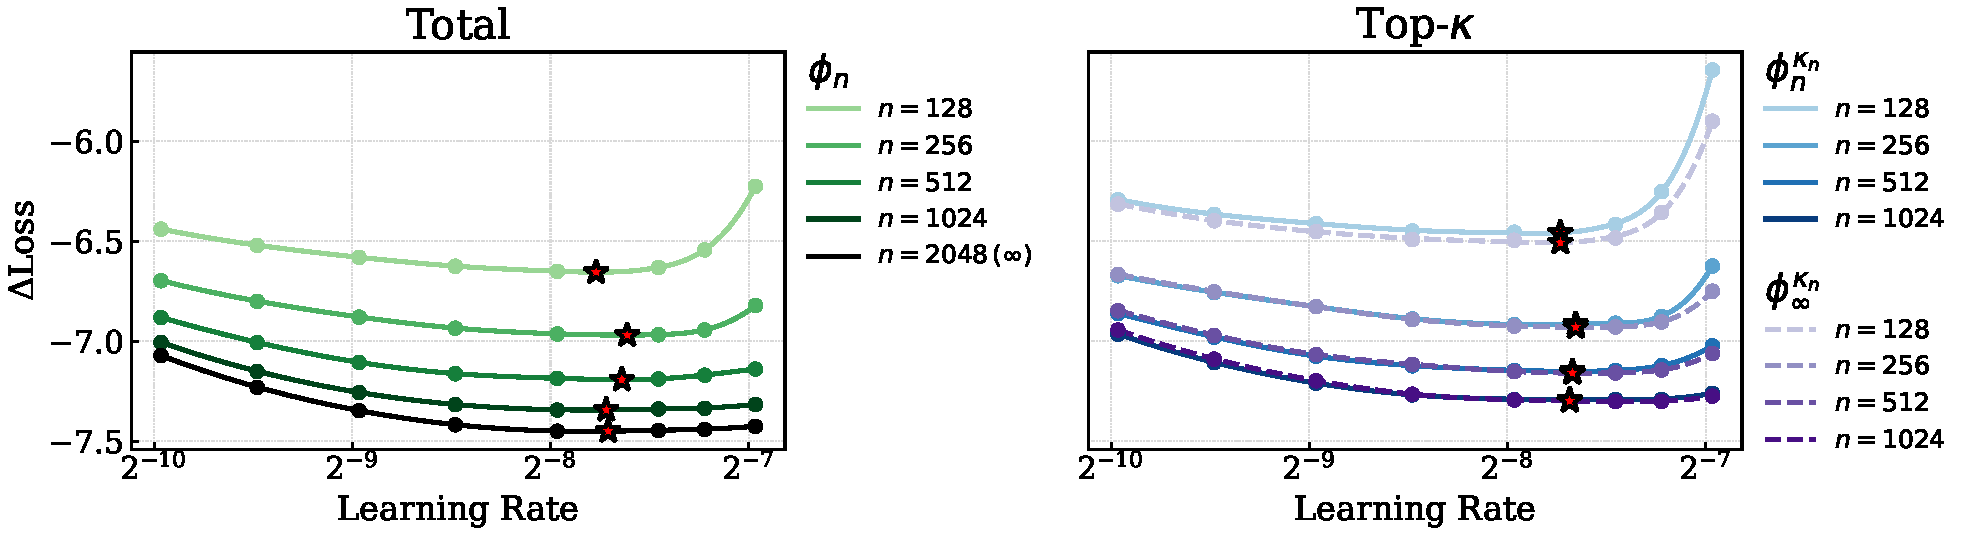
\includegraphics[width=0.95\linewidth]{arxiv_figures/ema_adam_lr_dynamic_k_perdim_topk_total_step_7185.pdf}
    \vspace{-2mm}
    \caption{\small \textbf{Left:} Total loss curves $\phi_n$ across widths. \textbf{Right:} Top-$\hptrunc_n$ loss curve pairs $\phi_n^{\hptrunc_n}$ (blue dashed) and $\phi_\infty^{\hptrunc_n}$ (purple dashed). The top-$\hptrunc_n$ pairs nearly overlap, with minimizers close to those of the corresponding total losses.}
    \label{fig:top_k_across_widths}
\end{figure}
\begin{figure}[!htb]
\vspace{-2mm}
    \centering
    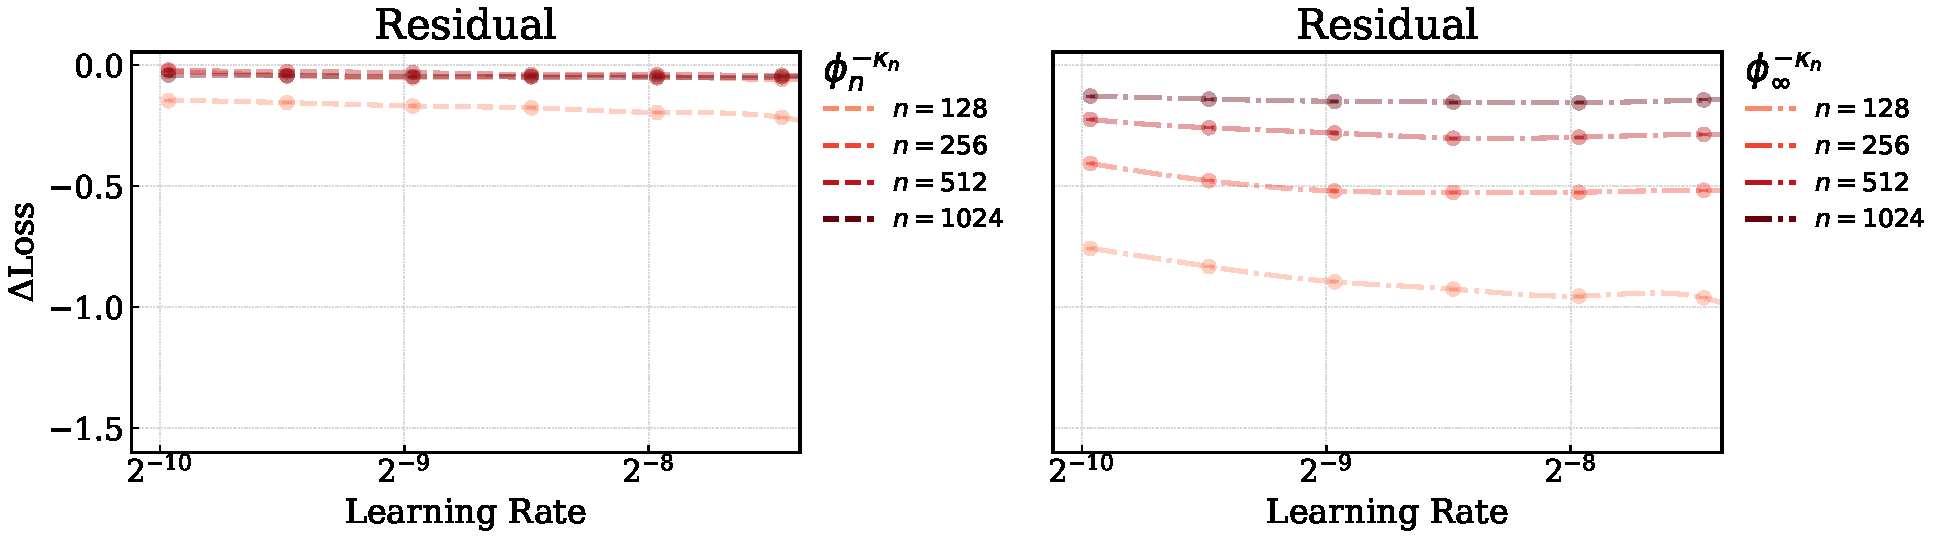
\includegraphics[width=0.95\linewidth]{arxiv_figures/ema_adam_lr_dynamic_k_perdim_residuals_step_7185.pdf}
    \vspace{-2mm}
    \caption{\small Residual losses are flat around the top-$\hptrunc_n$ minimizers, indicating less sensitivity to the learning rate.}
    \label{fig:resids_across_width}
    \vspace{-3.5mm}
\end{figure}


\paragraph{Decomposition Over Time.} Figure~\ref{fig:split-loss-over-time-step-7185} displays the top-$k$ loss with $k = 60$ and the residual loss over training, across multiple widths, at a fixed learning rate. We see that throughout training, the top-$k$ loss is nearly width-invariant and accounts for the majority of loss reduction. This indicates that the bulk of the improvement due to optimization comes from a low-dimensional subspace, and the benefit of width mostly comes from improving the residual loss. Accordingly, the ``width-dependent'' learning largely occurs in the tail components (and their contribution becomes more pronounced later in training). 

\paragraph{Decomposition Across Widths.} To evaluate our fast transfer conjecture, we apply our loss decomposition across widths and compute $\hptrunc_n = \hat{\hptrunc}(n)$ using Algorithm \ref{alg:compute-hptrunc-all}. We use the largest width $n_{\max} = 2048$ as an infinite-width proxy, and consider transfer from finite widths $n < n_{\max}$ to this proxy. In the right panel of Figure~\ref{fig:top_k_across_widths}, we see that the top-$\hptrunc_n$ loss curves nearly overlap across learning rates, i.e., $\phi_n^{\hptrunc_n} \approx \phi_\infty^{\hptrunc_n}$, despite the large gap in the total losses $\phi_n$ and $\phi_\infty$ shown in the left panel. Furthermore, the minimizers of the total loss are largely determined by the minimizers of the respective top-$\hptrunc_n$ loss, in the sense that both $\bhp_{\hptrunc_n}^\star(n) \approx \bhp^\star(n)$ and $\bhp_{\hptrunc_n}^\star(\infty) \approx \bhp^\star(\infty)$ (see Eq.\ (\ref{eq:decomposition_quantities})). In Figure \ref{fig:resids_across_width} we plot the corresponding residuals and see that they are flatter than the top-$\hptrunc_n$ losses in a neighborhood of the corresponding top-$\hptrunc_n$ minimizer. As a result, the residuals contribute less to the determination of the overall optimal learning rate.


\begin{figure}[t]
\vspace{-3mm}
    \centering
    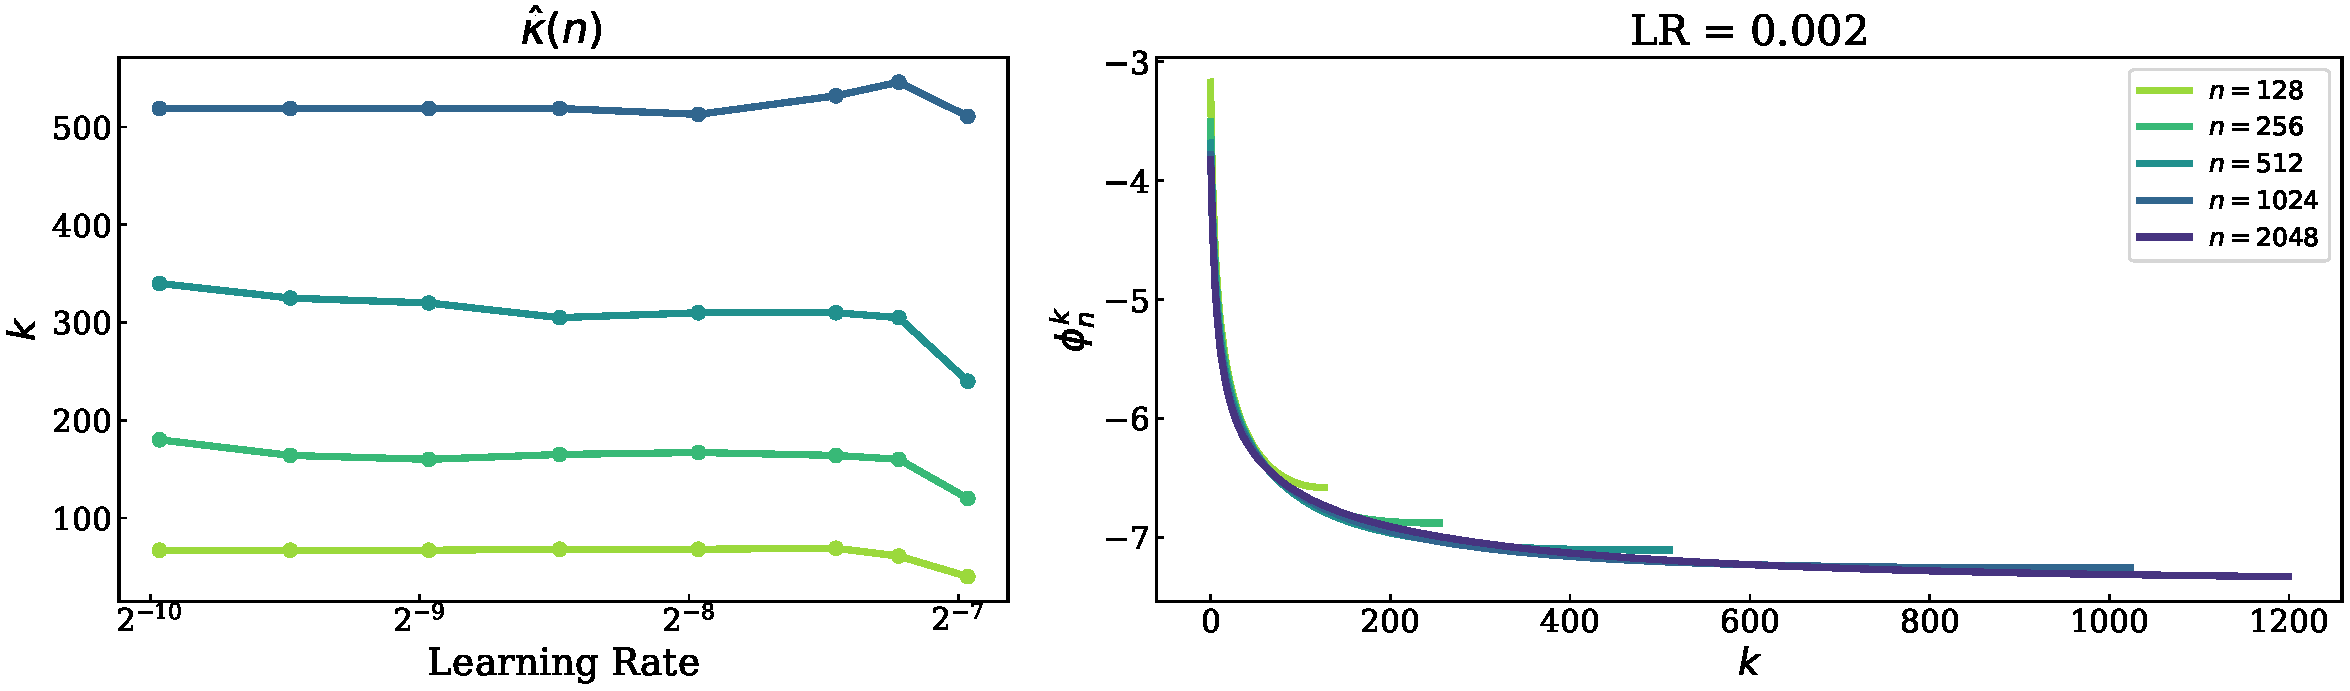
\includegraphics[width=0.88\linewidth]{arxiv_figures/ema_adam_lr_kvec_step_7185.pdf}
    \vspace{-1.5mm}
    \caption{\small \textbf{Left:} Computed values of $\hat{\hptrunc}(n)$ using Algorithm \ref{alg:compute-hptrunc-all}. \textbf{Right:} Top-$k$ losses $\phi_n^k$ for $\mathrm{LR}=0.002$, which descend rapidly with $k$ and overlap across widths over an intermediate range where top-$k$ invariance holds.}
    \label{fig:adam_topk_profile}   
    \vspace{-1mm}
\end{figure}

\paragraph{Top-$k$ Profile.} To further interpret the decomposition and the computed values $\hat{\hptrunc}(n)$, we now examine Figure \ref{fig:adam_topk_profile}. The left panel shows the computed values of $\hat{\hptrunc}(n)$, which are approximately constant across learning rates and grow sublinearly with $n$. The right panel plots $\phi_n^k$ for a fixed learning rate as a function of $k$. The top-$k$ loss varies smoothly with $k$, dropping rapidly at first and then flattening out. Notably, we can see that $\hat{\hptrunc}(n)$ is chosen roughly at the index $k$ where the curve $\phi_n^k$ ``peels off'' from the $\phi_{\infty}^k$ curve. This index marks the transition where increasing $k$ starts to include width-sensitive directions and balances the tradeoff discussed at the end of Section \ref{sec:topk_decomposition}. We see in the figure that this transition point increases with $n$ since the finite-width model shares more converged components with the infinite-width proxy. Consequently, $\hat{\hptrunc}(n)$ increases with $n$, and the residual $\phi_\infty^{-\hptrunc_n}$ shown in the right panel of Figure~\ref{fig:resids_across_width} decreases in magnitude. This differs from Figure~\ref{fig:split-loss-over-time-step-7185}, where we fixed $k = 60$ to isolate a width-invariant index and the residual magnitude grew with $n$. Compared to the infinite-width residual, the finite-width residual $\phi_n^{-\hptrunc_n}$ is smaller since there are fewer tail components, hence the curves in the left panel of Figure~\ref{fig:resids_across_width} are closer to zero.


Overall, we can qualitatively see how our decomposition can account for fast transfer in the sense described in Section~\ref{sec:fast-transfer}, even when the convergence of the loss itself is much slower. The provides concrete evidence for our central hypothesis that there is a low-dimensional projection of the trajectory which remains nearly invariant across width and is responsible for deciding the learning rate. 
In Appendix \ref{app:gpt_adam_lr}, we observe similar fast-transfer behavior for GPT-2 architecture trained on FineWeb~\citep{penedo2024fineweb} using Adam. 

\begin{figure}[b]
\vspace{-6mm}
    \centering
    \begin{subfigure}[t]{0.49\linewidth}
        \centering
        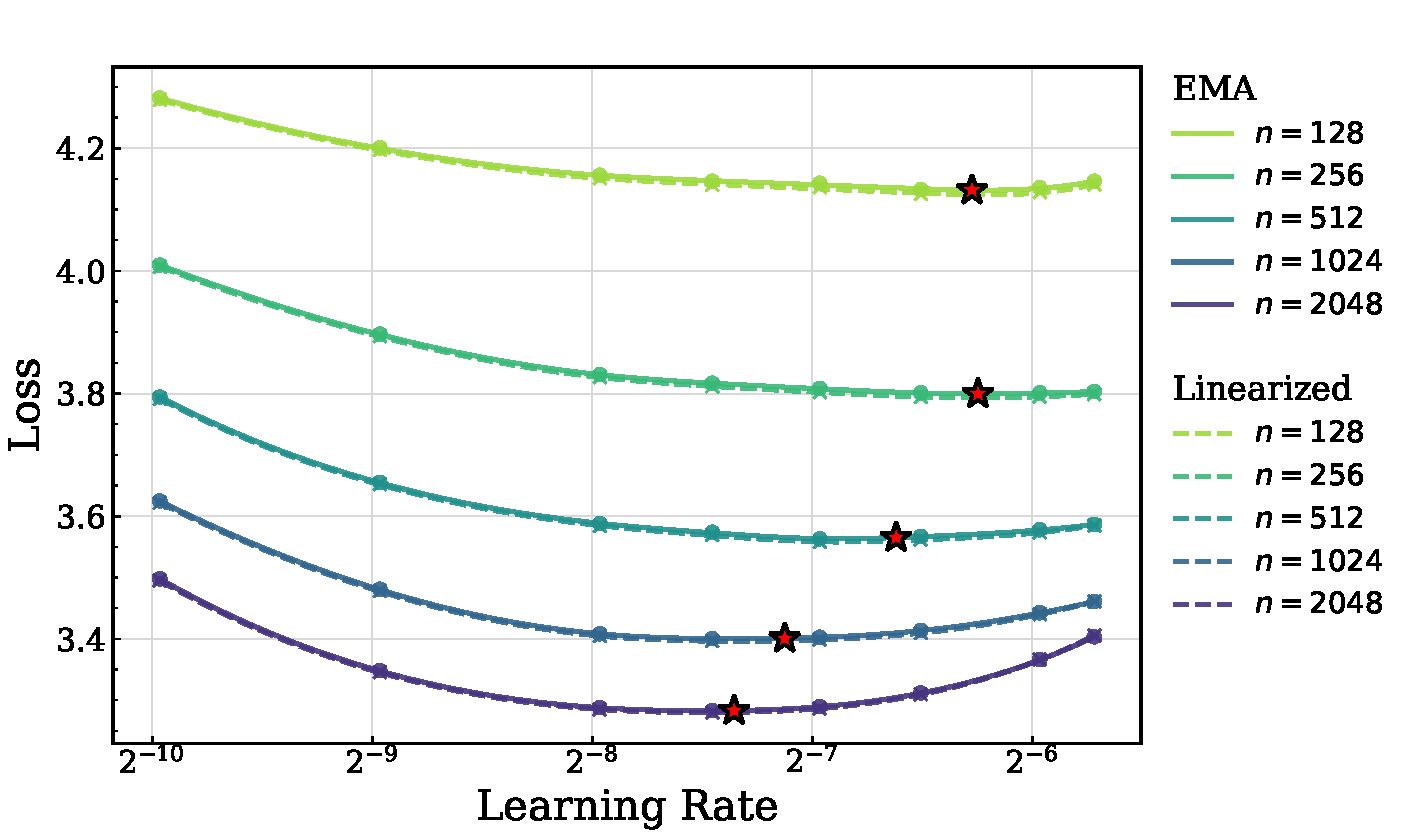
\includegraphics[width=\linewidth]{arxiv_figures/ema_muon_lr_step_7185.pdf}
        \caption{EMA loss (solid) and linearized loss (dashed).}
        \label{fig:ema_muon_lr_step_7185}
    \end{subfigure}
    \hspace{2.5mm}
     \begin{subfigure}[t]{0.4\linewidth}
        \centering
        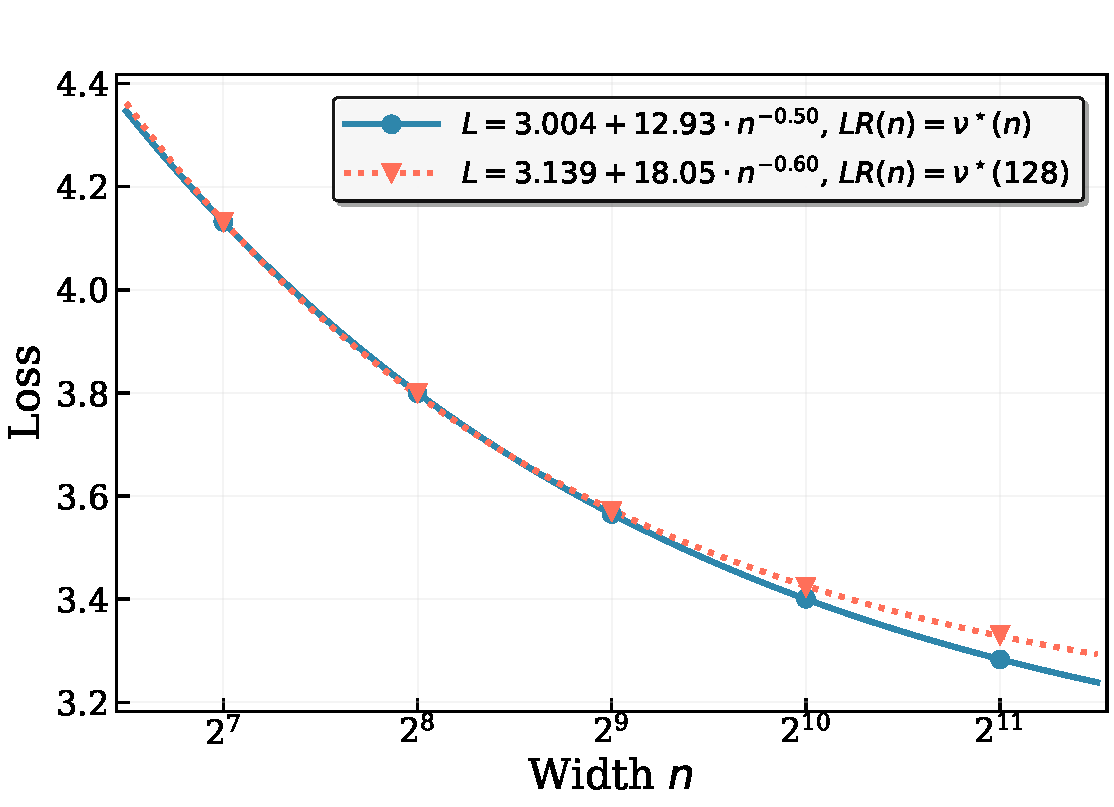
\includegraphics[width=\linewidth]{arxiv_figures/overlay_ema_muon_step_7185.pdf}
        \caption{Scaling law for the EMA loss.}
        \label{fig:ema_muon_step_7185_scaling_law}
    \end{subfigure}
    \caption{\small Same model and dataset as Fig.\ \ref{fig:ema_llama_step_7185}, but trained with Muon. \textbf{Left:} EMA and linearized losses coincide. \textbf{Right:} EMA loss versus width $n$ for the learning rate choices $\hp^\star(n)$ [blue dots] and $\hp^\star(128)$ [orange triangles]. At large $n$, using $\hp^\star(128)$ becomes suboptimal, indicating imperfect transfer.}
    \vspace{-2mm}
    \label{fig:ema_llama_step_7185_muon}
\end{figure}

\subsubsection{Llama with Muon}\label{sec:llama_muon} 

We repeat the same experiments in Section \ref{sec:llama_adam} but using the recently popularized Muon optimizer~\citep{jordan2024muon}, which updates the model weights via the orthogonalized momentum gradients (see Appendix \ref{app:llama_muon} for details). Figure~\ref{fig:ema_muon_lr_step_7185} shows that the optimal learning rate shift is more pronounced with Muon than with Adam (see Figure \ref{fig:ema_adam_lr_step_7185}). This larger shift leads to suboptimal performance at larger widths when using transferred hyperparameters, as demonstrated in Figure~\ref{fig:ema_muon_step_7185_scaling_law}: the scaling law using the transferred hyperparameter diverges noticeably from the one using the optimal hyperparameters. While this transfer suboptimality is offset by the improved overall performance of Muon, it is still an interesting example of ``imperfect'' transfer, and our decomposition reveals distinctive properties of Muon's learning dynamics. 

\begin{wrapfigure}{r}{0.44\textwidth}  
\vspace{-3.6mm} 
    \centering
    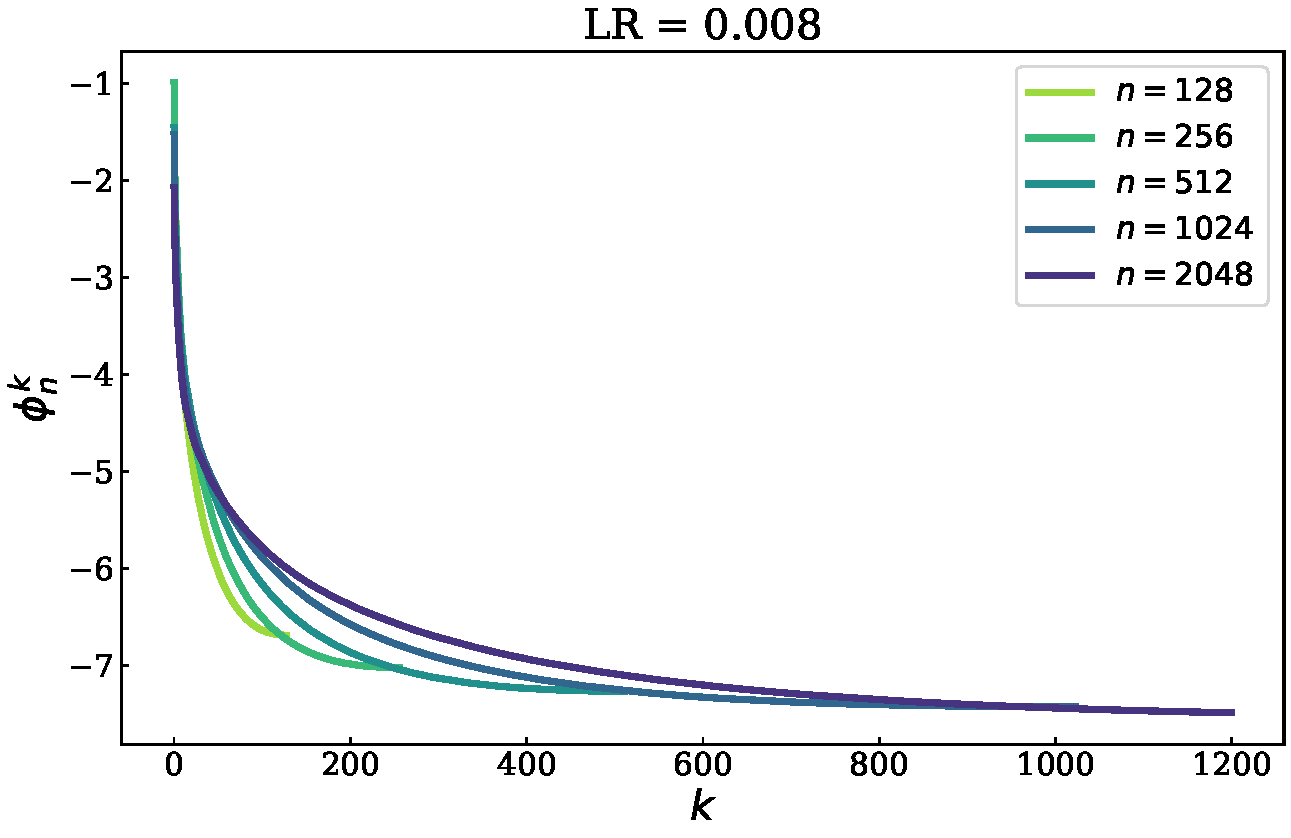
\includegraphics[width=0.43\textwidth,keepaspectratio]{arxiv_figures/ema_muon_lr_topk_profile.pdf}
    \vspace{-2mm}
    \caption{\small Top-$k$ losses $\phi_n^k$ for Muon. The curves descend and flatten out slowly with $k$, especially for large $n$, showing that top-$k$ invariance holds only for a narrow range of $k$ and the residual is significant.}
    \label{fig:muon_topk_profile}
    \vspace{-2mm}
\end{wrapfigure}

Figure \ref{fig:muon_topk_profile} reveals that top-$k$ invariance holds only for small $k$ (up to $k_0 \approx 10$). 
This is in sharp contrast with the decomposition for Adam (Figure~\ref{fig:adam_topk_profile}), in which we observe approximately invariant $\phi_n^k$ (up to $k \approx 60$) that explains a large fraction of the loss reduction. For $k > k_0$, we clearly see that $\phi_n^k$ increases with $n$, even though $\phi_n$ decreases with $n$. 
This indicates that under our layer-wise decomposition, Muon is ``spreading'' the loss decrease over more directions: each direction contributes less, but the cumulative decrease over all directions is larger since $\phi_n$ decreases with $n$. Intuitively speaking, this lack of low-dimensional invariance is connected to the ``whitening'' step in Muon which increases the effective rank of the gradient \citep{frans2025really,davis2025spectral}. Consequently, the low-rank structure in Adam and SGD updates that enables fast transfer may not be present in full-matrix preconditioned updates. 



In Appendix \ref{app:gpt_muon_lr}, we report the learning rate transfer of Muon in a different problem setting: training GPT-2 on the FineWeb dataset. 
There again we find that Muon displays a less stable optimal learning rate across widths, but due to the flatness of the overall loss, the transfer performance is still nearly optimal. 
Interestingly, in Figure~\ref{fig:ema_muon_lr_multiple_topk_profile} we observe that the decomposition looks qualitatively different for different learning rates. In particular, while the small learning rate decomposition resembles that in our earlier Muon experiment (Figure~\ref{fig:muon_topk_profile}), at near-optimal learning rates we instead see more pronounced top-$k$ invariance that is closer to the Adam decomposition (Figure~\ref{fig:adam_topk_profile}). 
We speculate that this can happen when the dynamics of the layers trained with AdamW (e.g., the input and output layers, see Appendix~\ref{app:muon}) tend to dominate at certain learning rates, but we leave careful verification of this to future work. In any case, this example highlights that the correct notion of invariance for Muon is subtle and can be hyperparameter dependent. 

\paragraph{Experiment with Muon Variants.} 
To investigate the effect of whitening on learning rate transfer and the decomposition in a more controlled manner, in Appendix~\ref{app:dion} we perform the same experiment using the Dion optimizer~\citep{ahn2025dion}, which has a rank hyperparameter controlling the dimension of the whitened subspace. If we choose the Dion rank to be small, we expect a higher degree of invariance and less influence of the residual, which should lead to improved transfer. In Figure~\ref{fig:ema_llama_step_7185_dion_bounded_rank}, we see that setting the rank equal to $\min(n/2, 128)$ indeed greatly improves transfer compared to using a rank of $n/2$, which closely resembles the Muon results (Figure~\ref{fig:ema_llama_step_7185_muon}). Perhaps surprisingly, although Dion with bounded rank does exhibit more stable transfer, the resulting top-$k$ decomposition (Figure~\ref{fig:ema_dion_bounded_rank_lr_topk_profile}) is more Adam-like, but still looks qualitatively similar to that for Muon. We speculate that there exists a different notion of invariance\footnote{For example, it could make sense to consider invariance for the \emph{rescaled} top-$k$ loss $\tilde{\phi}_n^k := \phi_{n}^{m_n(k)}$ where $m_n(k) = \alpha k n^{\beta}$ for some $\alpha > 0$, $\beta \in (0, 1)$ and $k \in [n^{1-\beta} / \alpha]$, since this would capture an increasing number of directions with $n$. \vspace{-3.5mm} } for optimizers like Muon and Dion, obtained by modifying our proposed decomposition, that leads more cleanly to a qualitative picture similar to what we see for SGD and Adam; for such suitable notion of invariance, we expect the corresponding residual loss will be flatter for Dion with bounded rank compared to Muon. 

\subsubsection{MLP with SGD}\label{sec:mlp_sgd}
For a setting with a new data modality and architecture, we now consider learning rate transfer in two-layer MLPs trained on CIFAR-10 using momentum SGD. Additional details can be found in Appendix \ref{app:mlp_sgd}. 
This setting will have the benefit of being lightweight enough to support a detailed analysis and interpretation of our decomposition from a \textit{data-centric} point of view (similar in spirit to \citet{zhong2021larger,kaplun2022deconstructing,ilyas2022datamodels}). 
In Figure \ref{fig:ema_sgd_step_9695} we can see that our linearization described in Section \ref{sec:topk_decomposition} is accurate and the optimal HP is stable across width (though transfer is ``imperfect'' compared to Figure \ref{fig:ema_llama_step_7185}). 
We also observe that the benefit of width is less pronounced compared to the language setting and that loss convergence occurs at a faster rate of approximately $n^{-0.77}$. This aligns with the intuition that CIFAR-10 is a ``simpler'' task; in Appendix \ref{app:mlp_sgd} we further support this intuition through the top-$k$ decomposition (Fig.~\ref{fig:sgd_kvec}). 

\begin{figure}[t]
\vspace{-4mm}
    \centering
    \begin{subfigure}[t]{0.49\linewidth}
        \centering
        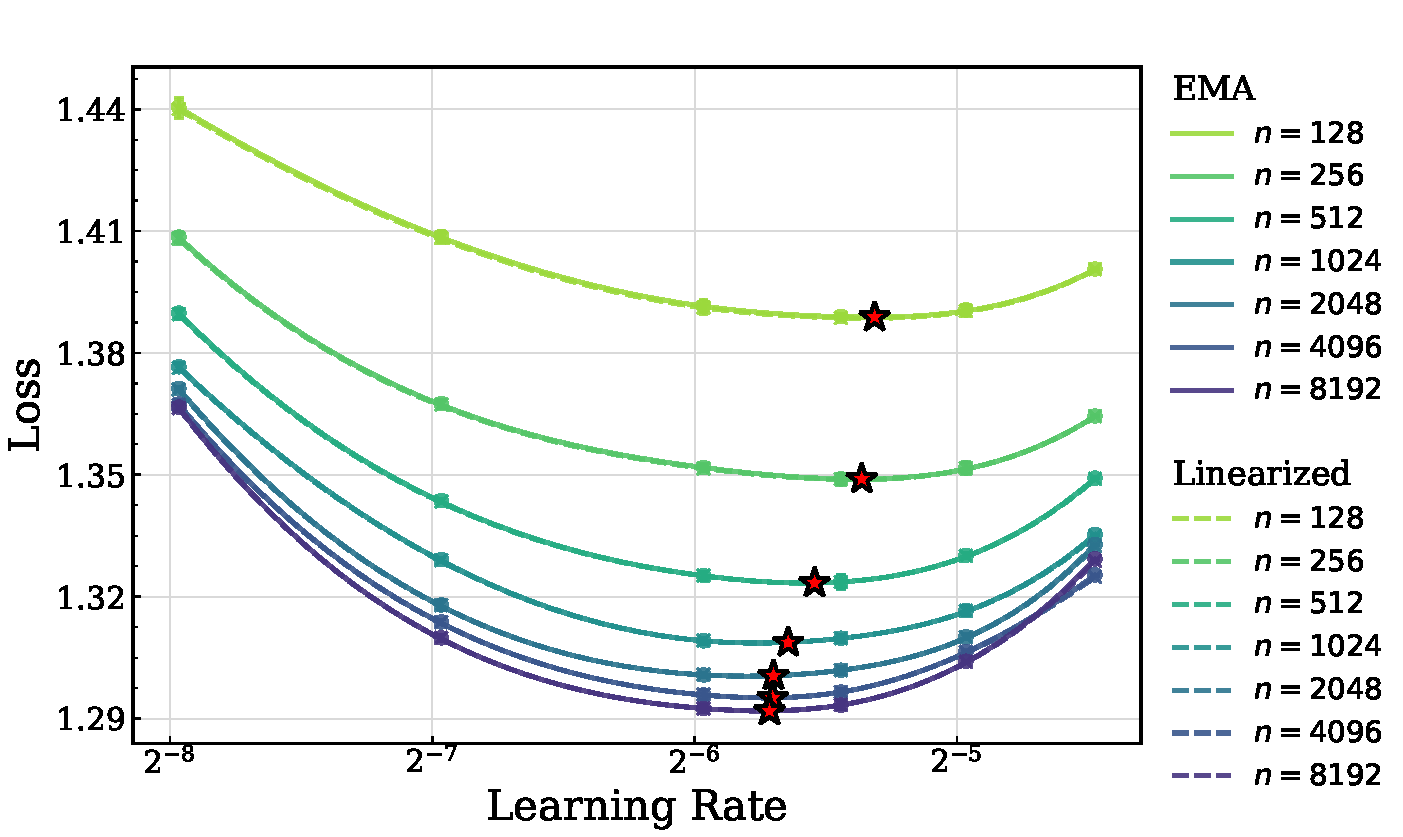
\includegraphics[width=\linewidth]{arxiv_figures/ema_sgd_lr_step_9695.pdf}
        \caption{The final EMA loss (solid) and final linearized.}
        \label{fig:ema_sgd_lr_step_9695}
    \end{subfigure}
    \hspace{2.5mm}
    \begin{subfigure}[t]{0.4\linewidth}
        \centering
        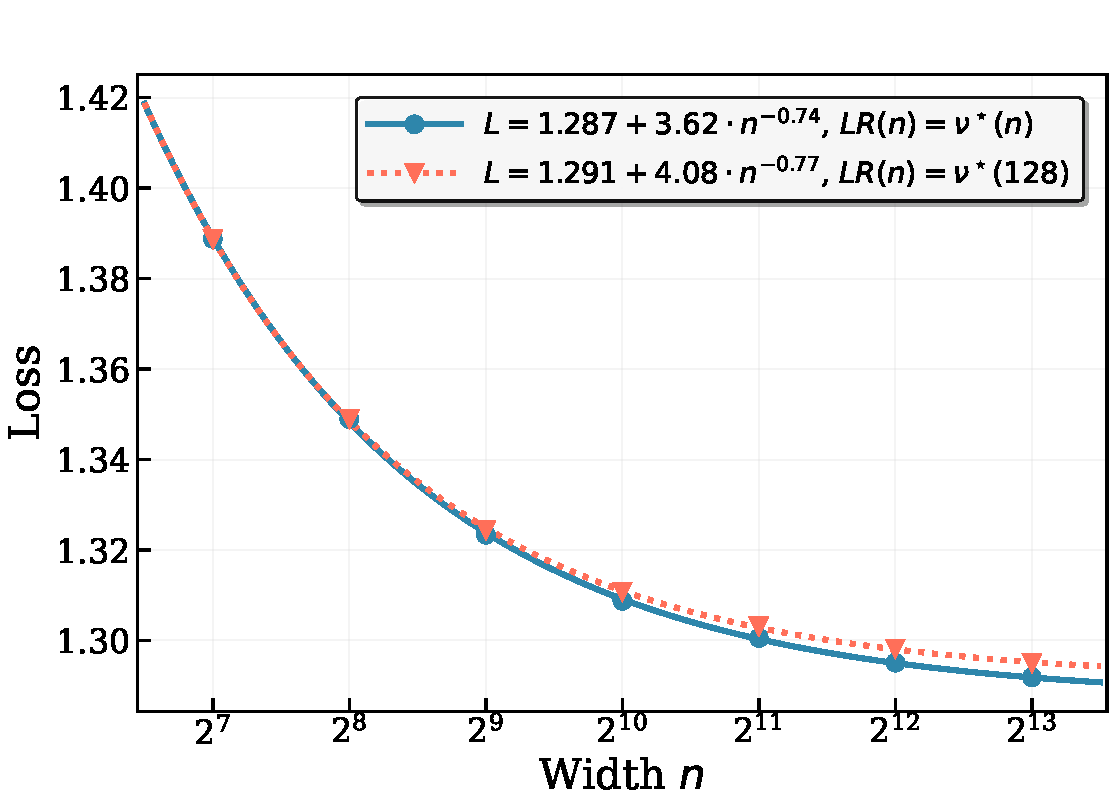
\includegraphics[width=\linewidth]{arxiv_figures/overlay_ema_sgd_step_9695.pdf}
        \caption{Scaling law for the EMA loss.}
        \label{fig:ema_sgd_lr_step_9695_scaling_law}
    \end{subfigure}
    \vspace{-1mm}
    \caption{\small Two-layer MLP trained on CIFAR-10 using SGD. We observe reliable but imperfect transfer. \textbf{Left:} The EMA and linearized losses coincide. \textbf{Right:} EMA loss across widths using the width-dependent optimal learning rate $\hp^\star(n)$ [blue dots] and the fixed width-128 choice $\hp^\star(128)$ [orange triangles].}
    \vspace{-1mm}
    \label{fig:ema_sgd_step_9695}
\end{figure}


\paragraph{Sample-wise Decomposition.} We have previously seen that the top-$k$ components account for the majority of loss decrease, while the tail components account for the improved learning at larger widths. However, this picture does not shed light on what structures the top vs.~tail components are actually learning. To gain a better qualitative understanding, we now apply our decomposition at a sample-wise level and examine how different components affect the loss on each example. We conjecture the following structure:
\begin{itemize}[leftmargin=*,topsep=1mm]
    \item \textbf{Easy Examples:} Examples that are almost entirely learned by the \textit{top components} are ``easy'' examples. The loss on these examples will show fast transfer and essentially determine the optimal HPs.

    \item \textbf{Hard Examples:} Examples that rely on the \textit{tail components} are ``hard'' examples. These examples are learned differently across widths because tail components are not width-invariant, hence slowing transfer.
\end{itemize}

\begin{figure}[b]
\vspace{-1.25mm}
    \centering
    \begin{subfigure}[t]{0.37\linewidth}
        \centering
        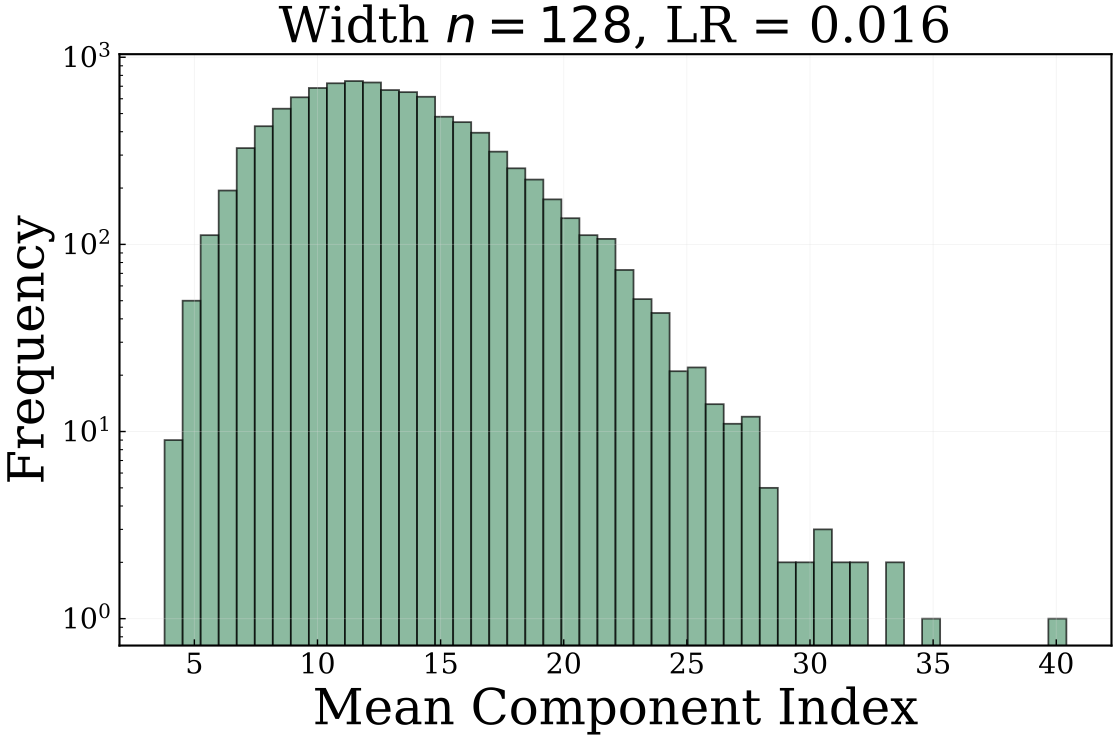
\includegraphics[width=\linewidth]{arxiv_figures/wp_128_histogram.png}
        \caption{Histogram of MCI (CIFAR-10).}
        \label{fig:wp_128_histogram}
    \end{subfigure}
    \hspace{2mm}
    \begin{subfigure}[t]{0.6\linewidth}
        \centering
        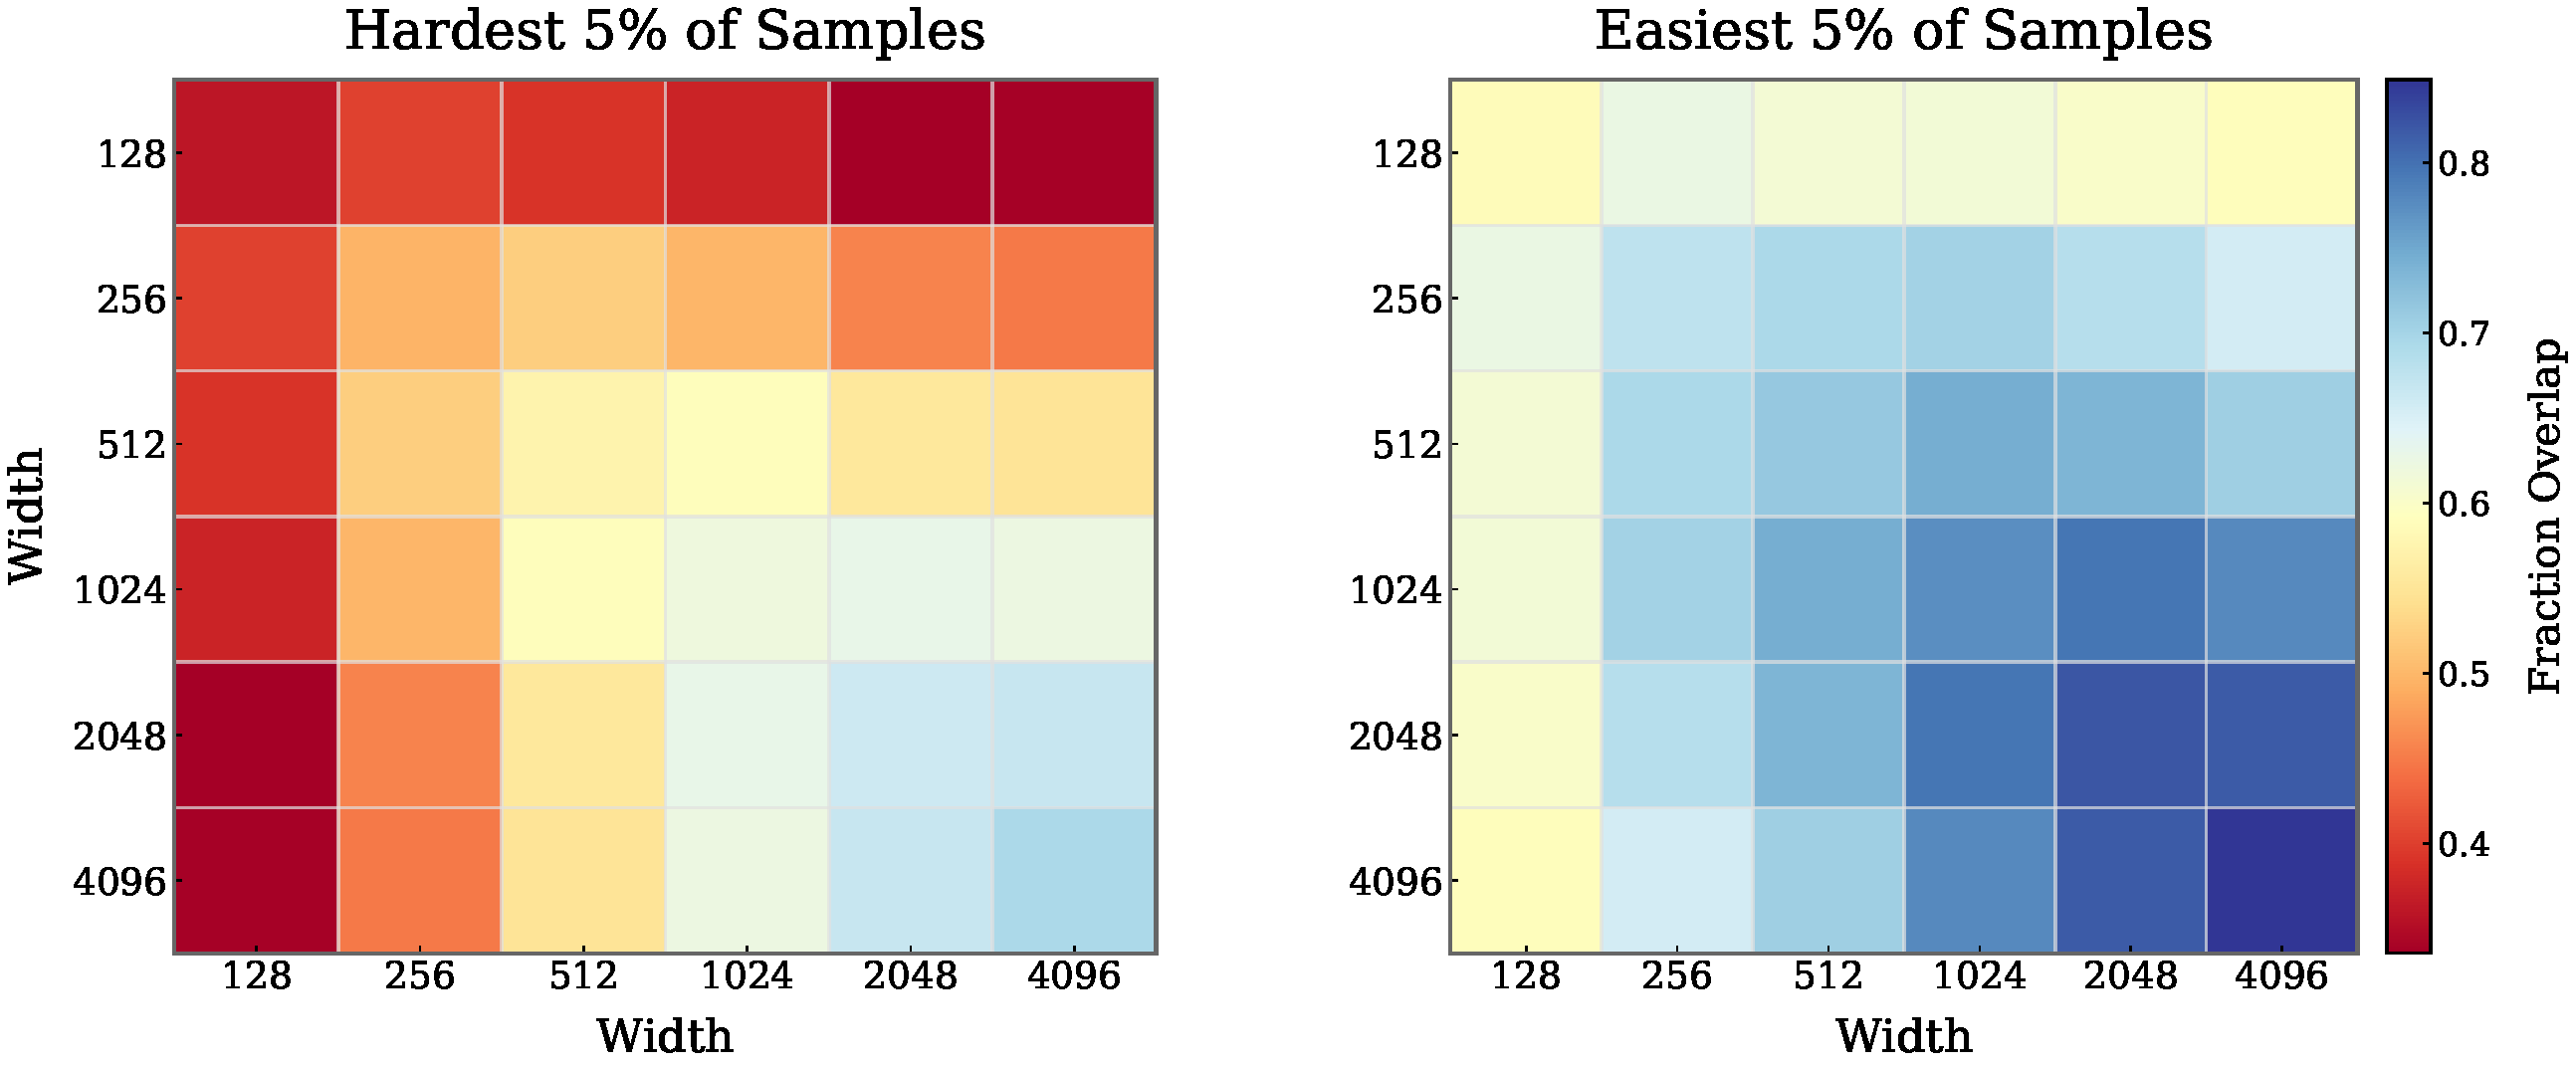
\includegraphics[width=\linewidth]{arxiv_figures/sample_overlap_lr_0.016.pdf}
        \caption{Consistency of top 5\% hardest and easiest examples.}
        \label{fig:sample_overlap}
    \end{subfigure}
    \vspace{-1mm}
    \caption{\small \textbf{Left:} $\MCI$ computed on CIFAR-10 for $n = 128$ and learning rate $0.016$. The distribution is left-skewed with a small number of large outliers, indicating that most examples are ``easy''. \textbf{Right:} For each pair of widths and random seeds, we compare the sets of top or bottom 5\% of samples ranked by $\MCI_i$ and plot the average fraction of shared samples. Diagonal values need not be 1 since entries compare different seeds at the same width. Rankings are more stable for low-MCI (easy) examples and larger widths, and less stable for high-MCI examples and smaller widths.
    }
    \vspace{-3mm}
    \label{fig:histogram_overlap}
\end{figure}

\paragraph{Mean Component Index.} To make these notions precise, we now introduce a per-example statistic, the \textit{Mean Component Index} (MCI), which quantifies how much of the loss change for an example occurs in top versus tail components. 
Examples with small MCI correspond to the ``easy'' examples above and those with high MCI correspond to the ``hard'' examples. Let us recall the setup in Section \ref{sec:topk_decomposition}. For simplicity, let us consider a single layer $\bW$ with gradient $\bG$ and update $\delta \bW$ at time $t$, since everything will extend to multiple layers by summing over each layer. As before, let $\sym(\bG, \delta \bW)$ from Eq.\ (\ref{eq:alignmat}) be the alignment matrix between $\bG$ and $\delta \bW$ with eigenvalues $\lambda_1, \ldots, \lambda_n$ ordered such that $|\lambda_1| \geq \dots \geq |\lambda_n|$ and corresponding eigenvectors $\bu_1, \ldots, \bu_n$. The eigenvectors $\bu_j$ define the component directions in our decomposition. 
If we have $P$ data points and the loss $\mathcal{L}$ is the average over pointwise losses $\ell_i$ with gradients $\bG_i$, then $\bG$ is the average over $\bG_i$ and we can decompose $\delta \phi(\bW) = \inner{\bG}{\delta \bW}$ into
\[
    \delta \phi(\bW) = \inner{\bG}{\delta \bW} = \frac{1}{P} \sum\limits_{i=1}^P \inner{\bG_i}{\delta \bW} = \frac{1}{P} \sum\limits_{i=1}^P \sum\limits_{j=1}^n \bu_j^\top \bG_i^\top \delta \bW \bu_j = \frac{1}{P} \sum\limits_{i=1}^P \sum\limits_{j=1}^n (\delta \psi)_{ij},
\]
where we define $(\delta \psi)_{ij} := \bu_j^\top \bG_i^\top \delta \bW \bu_j$ to be the instantaneous linearized loss change of sample $i$ in the $j$ component from updating parameter $\bW$. By summing $(\delta \psi)_{ij}$ over time steps $t$ and matrix layers we can define $\psi_{ij}$ to be the linearized loss change of sample $i$ in the $j$ component over the entire trajectory. The mean component index $\MCI_i \in [1, n]$ for example $i$ is then defined to be the quantity
\begin{equation}\label{eq:mean_component_index}
    \MCI_i := \sum\limits_{j = 1}^n j p_j,~~p_j := \textstyle\frac{|\psi_{ij}|}{\sum\limits_{k=1}^n |\psi_{ik}|}~~\text{ and }~~\psi_{ij} := \sum\limits_{\ell \in [L]} \sum\limits_{t=0}^{T-1} (\delta \psi)_{ij}[\bW_t^{(\ell)}].
\end{equation}
We use $\MCI_i$ as a scalar index placing example $i$ along the easy-to-hard spectrum described above. 

\begin{figure}[b]
\vspace{-1mm}
\centering
\begin{subfigure}[t]{0.5\linewidth}
\centering
{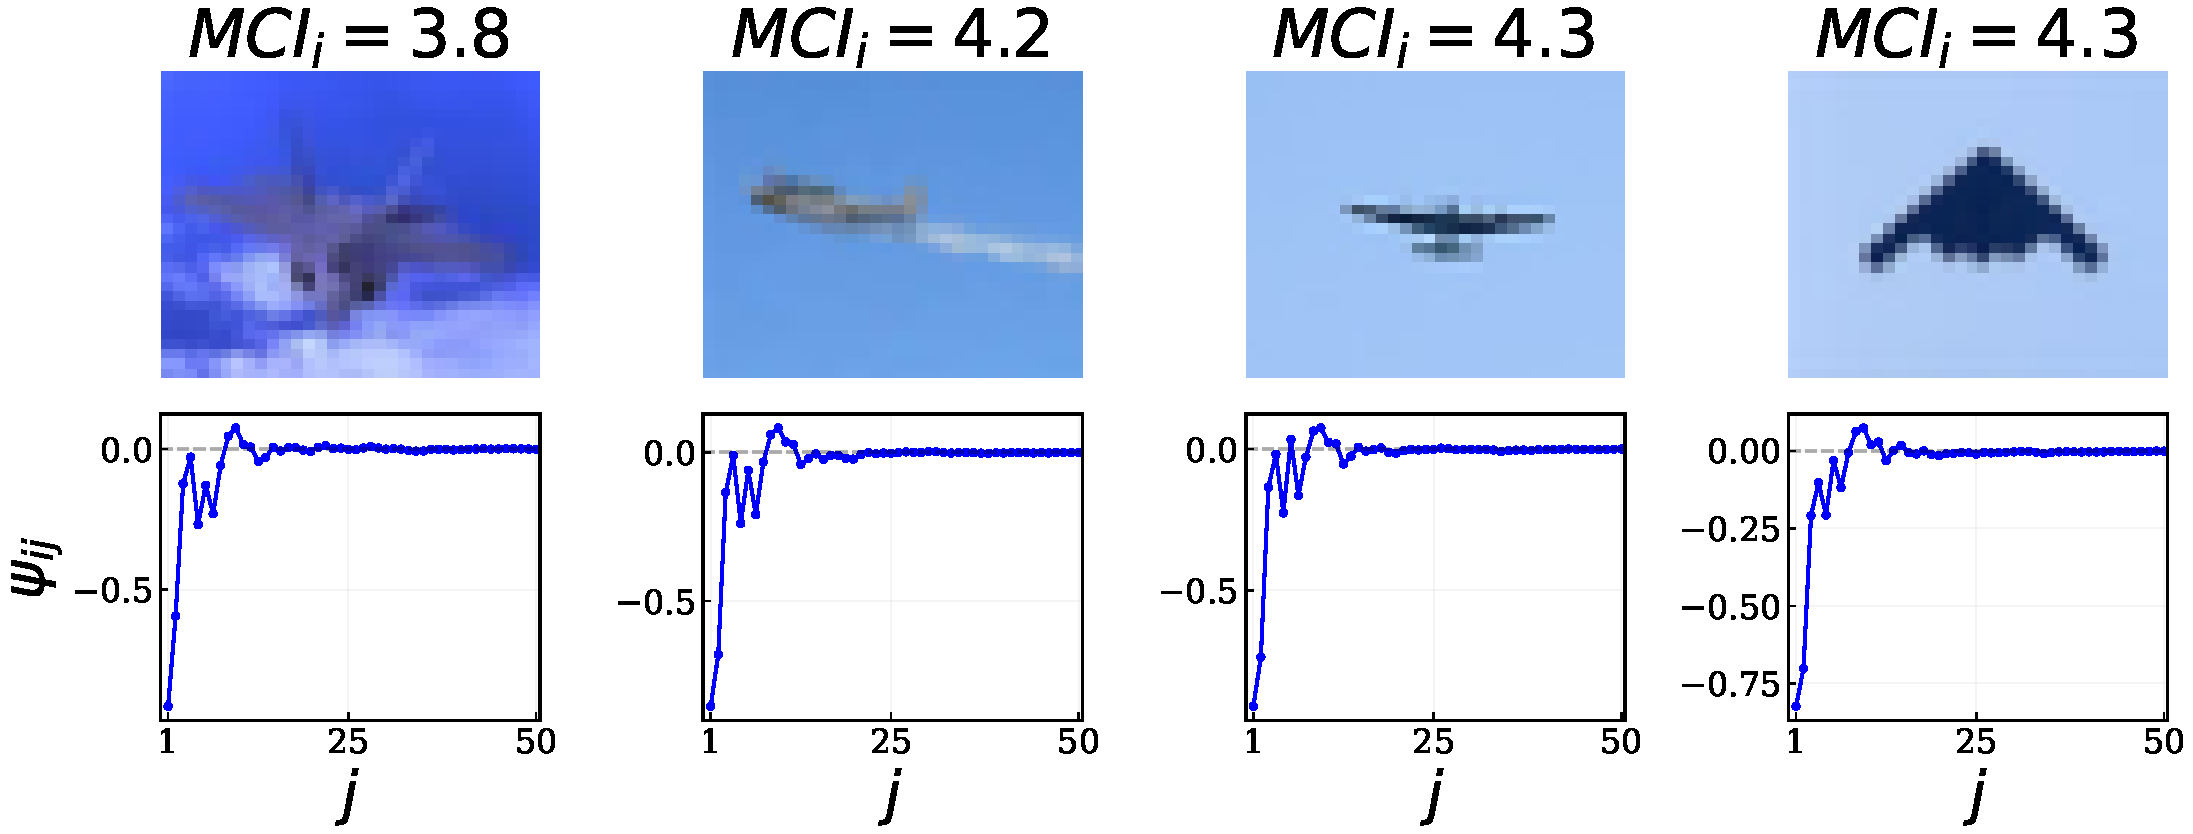
\includegraphics[width=0.98\textwidth]{arxiv_figures/sample_128_lowest.pdf}}  \vspace{-1.mm}
\caption{\small Lowest Mean Component Index (``easy'' samples).}
\label{fig_sample_128_easy}
\end{subfigure}%
\begin{subfigure}[t]{0.5\linewidth} 
\centering 
{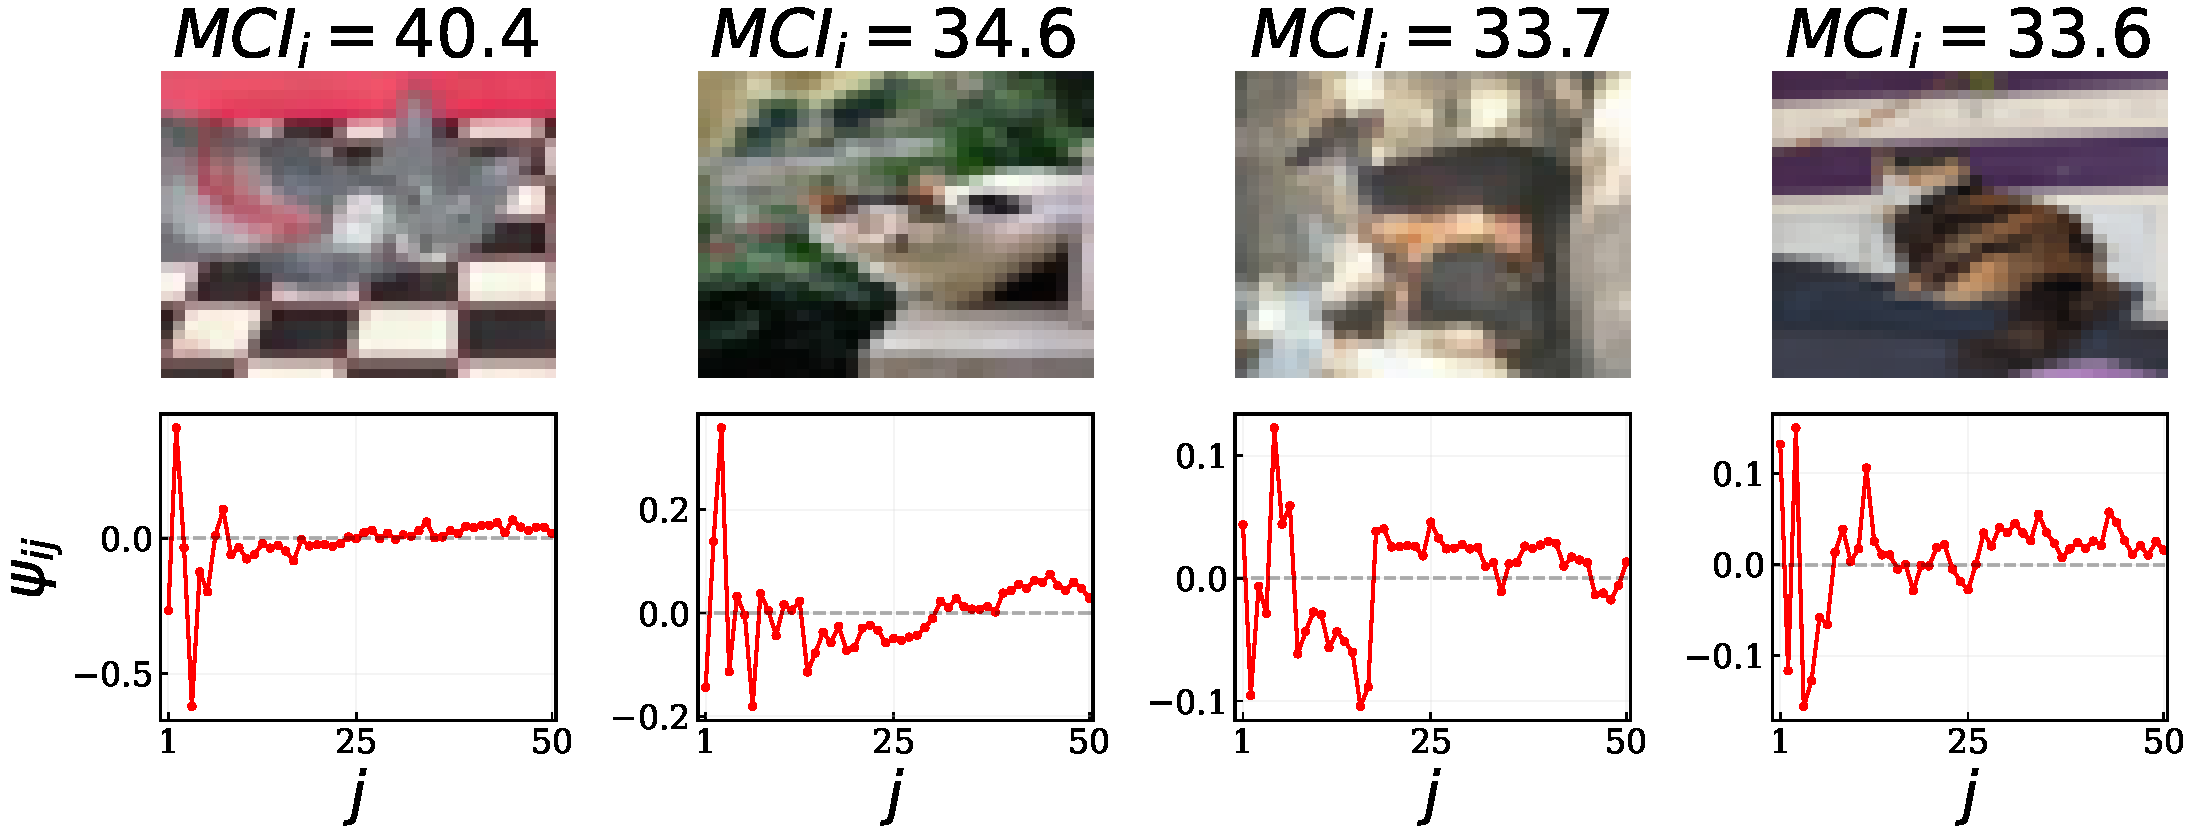
\includegraphics[width=0.98\textwidth]{arxiv_figures/sample_128_highest.pdf}} \vspace{-1.mm}
\caption{\small Highest Mean Component Index  (``hard'' samples).} 
\label{fig_sample_128_hard}
\end{subfigure}%
\vspace{-1mm}
    \caption{\small The five examples in CIFAR-10 validation set with lowest (left) and highest (right) MCI for a two-layer MLP of width $n = 128$ trained with SGD using LR = 0.016. 
    \textbf{Top row:} We visualize the samples and the corresponding MCI. \textbf{Bottom row:} We plot the $\psi_{ij}$ values for the first $50$ components $j$ (see Eq.\ (\ref{eq:mean_component_index})). 
    % The majority of the loss change is in component $j = 1$. 
    Note that the low-MCI examples turn out to be simple images from the airplane class which are learned early in training using simple features, while the high-MCI images are complex examples from different classes which are not learned well by the model.}
    \label{fig:sample_128}
    \vspace{-1.5mm}
\end{figure}


\paragraph{Empirical Findings.} In Figure \ref{fig:wp_128_histogram} we show the distribution of $\MCI_i$ for a network of width $n = 128$. The average $\MCI_i$ is about $12.9$, which is much smaller than $n$, and the distribution is left-skewed. This indicates that most samples are learned mainly through the top components, consistent with Figures \ref{fig:sgd_kvec} and \ref{fig:sgd_resids_across_widths}. 

In Figure \ref{fig:sample_128} we visualize the four examples with the smallest and largest MCI. Observe that examples with smallest MCI shown in Figure~\ref{fig_sample_128_easy} are visually simple (top panel) and are essentially learned by the first component (bottom panel) in our decomposition \eqref{eq:mean_component_index}, whereas the large MCI examples shown in Figure~\ref{fig_sample_128_hard} are more complex and require non-trivial contributions from tail components (i.e., $j>10$).  

Figure \ref{fig:sample_overlap} quantifies how similar the rankings of $\MCI_i$ over samples $i$ are across widths and random seeds. For widths $n_1, n_2$ and random seeds $s_1, s_2$, we take the top or bottom $5\%$ of samples ranked by MCI for each width and seed pair, giving us two subsets $S_1$ and $S_2$ of $[P]$. For a given pair of widths we compute the fraction of overlap $|S_1 \cap S_2| / 0.05P$ and average over pairs of seeds $s_1$ and $s_2$, ignoring $s_1 = s_2$ if $n_1 = n_2$ since this would be trivially equal to one. We observe less agreement when $\min(n_1, n_2)$ is smaller and we restrict to samples with higher MCI, suggesting that easy (low-MCI) examples are learned more consistently at different widths and random seeds than hard (high-MCI) examples. 

\begin{figure}[!htb] 
\vspace{-5.5mm}
    \centering
    \begin{subfigure}[t]{0.48\linewidth}
        \centering
        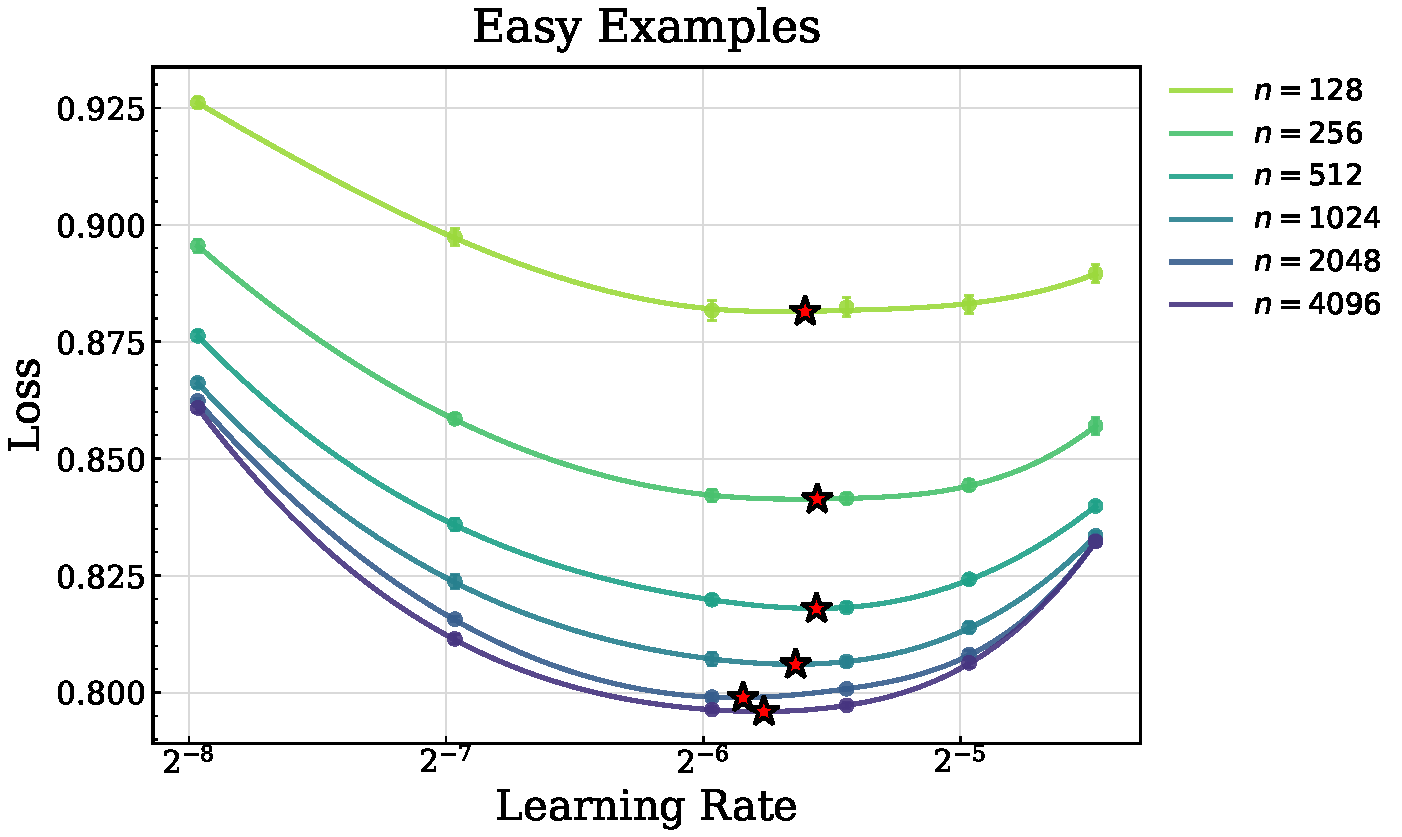
\includegraphics[width=\linewidth]{arxiv_figures/easy_examples.pdf}\vspace{-1mm}
        \caption{The final EMA loss (easy examples).}
        \label{fig:easy_examples_transfer}
        \vspace{2mm}
    \end{subfigure}
    \hspace{2.5mm}
    \begin{subfigure}[t]{0.4\linewidth}
        \centering
        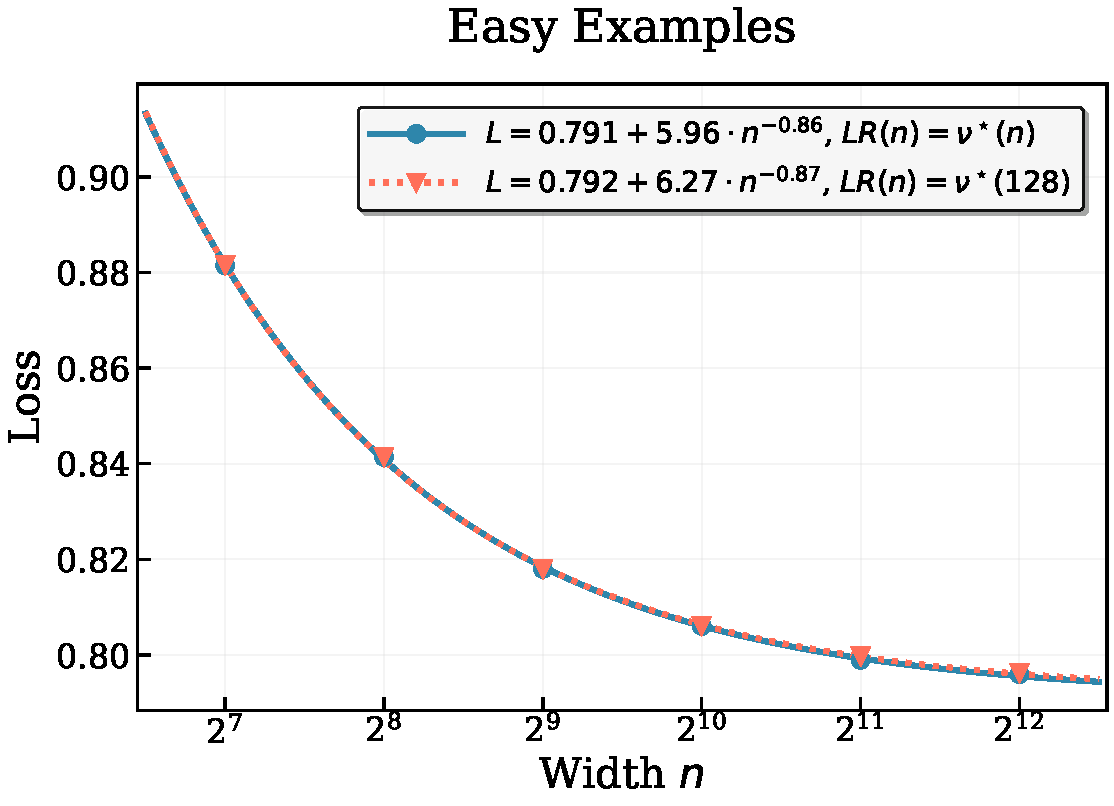
\includegraphics[width=\linewidth]{arxiv_figures/easy_examples_scaling_law.pdf}\vspace{-1mm}
        \caption{Scaling law for EMA loss (easy examples).}
        \label{fig:easy_examples_scaling_law}
            \vspace{2mm}
    \end{subfigure}
        \begin{subfigure}[t]{0.48\linewidth}
        \centering
        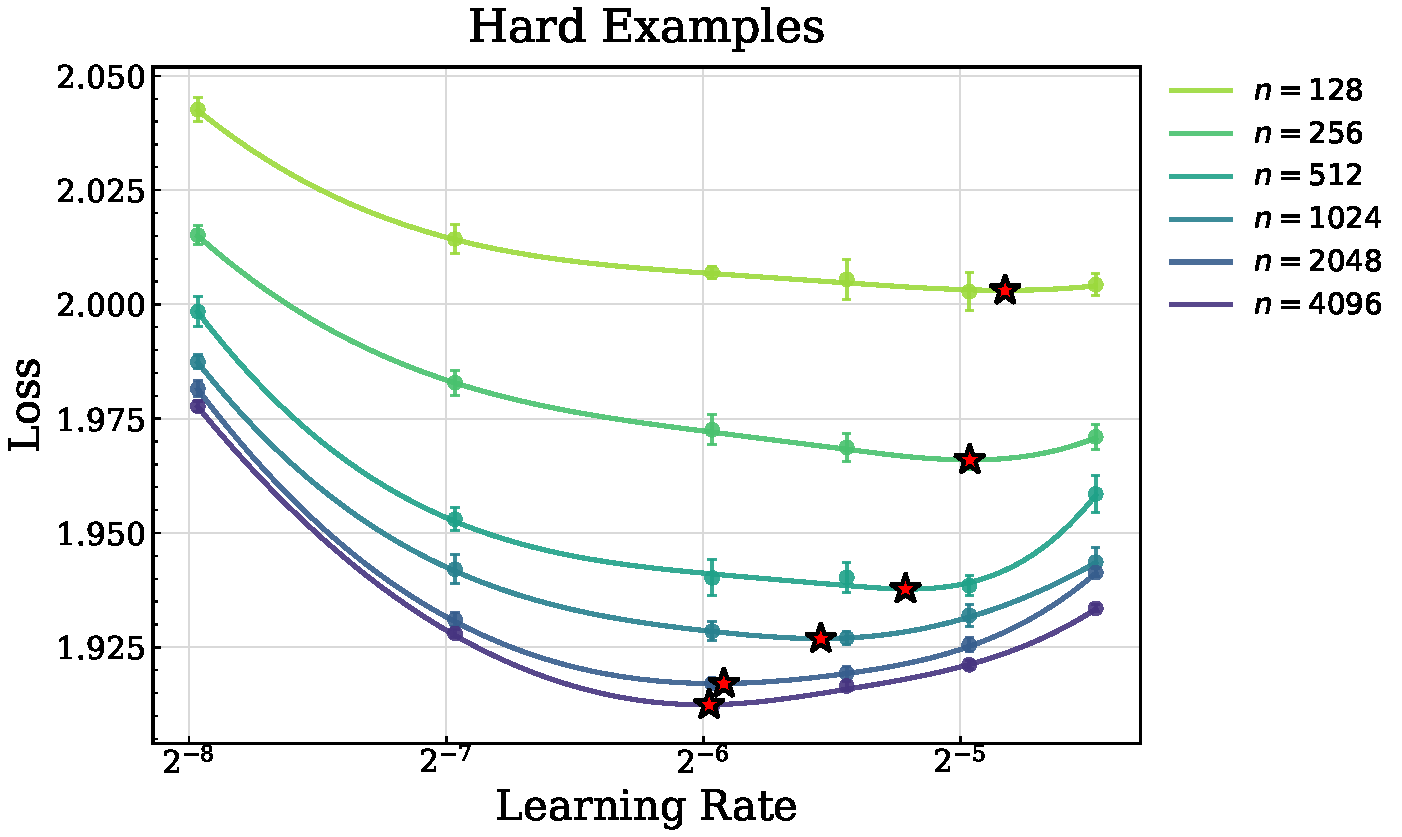
\includegraphics[width=\linewidth]{arxiv_figures/hard_examples.pdf}\vspace{-1mm}
        \caption{The final EMA loss (hard examples).}
        \label{fig:hard_examples_transfer}
    \end{subfigure}
    \hspace{2.5mm}
    \begin{subfigure}[t]{0.4\linewidth}
        \centering
        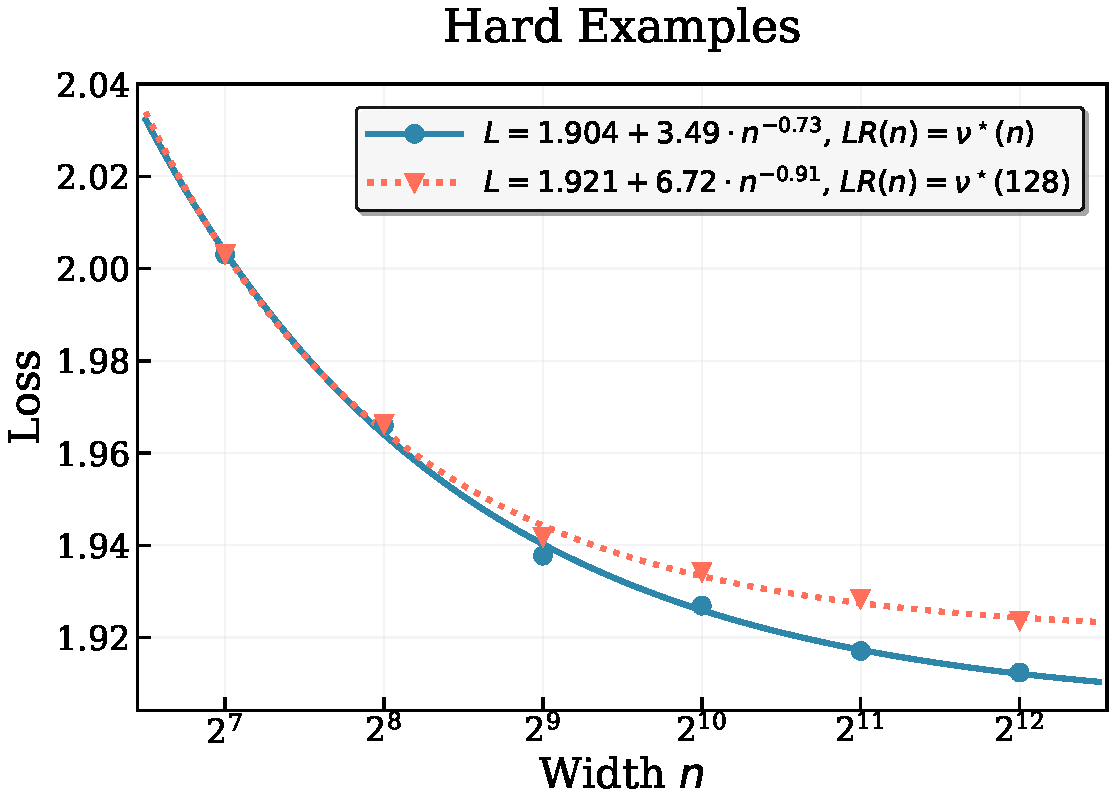
\includegraphics[width=\linewidth]{arxiv_figures/hard_examples_scaling_law.pdf}\vspace{-1mm}
        \caption{Scaling law for EMA loss (hard examples).}
        \label{fig:hard_examples_scaling_law}
    \end{subfigure}
    \vspace{-1mm}
    \caption{\small EMA loss on the 25\% easiest \textbf{(Top)} and 5\% hardest \textbf{(Bottom)} examples in the CIFAR-10 validation set, based on MCI computed on the width $n = 128$, LR = 0.016 model. Observe that for EMA loss on the easy subset, the optimal learning rates are well-aligned across widths and match the (large width) optimal HP on the full validation set (Figure \ref{fig:ema_sgd_lr_step_9695}), whereas the optimal learning rates for the hard subset shift significantly and yields suboptimal transfer. }
    \label{fig:examples_scaling_law}
    \vspace{-0.9mm} 
\end{figure}

Due to the consistency across scale observed in Figure~\ref{fig_sample_128_easy}, we intuitively expect the optimal learning rate for these easy examples to be stable and transferrable. 
Hence in Figure~\ref{fig:examples_scaling_law} we probe the effect of easy versus hard examples on learning rate transfer. Up to this point, all losses have been computed on the full validation set. To isolate the effect of individual data points, we now evaluate learning-rate sweeps on subsets of the validation set consisting only of easy or hard examples, based on the previously computed MCI values from training a single model of with $n = 128$. 
On the easy subset (lowest 25\% MCI) we see near-perfect transfer (Figures \ref{fig:easy_examples_transfer} and \ref{fig:easy_examples_scaling_law}), and the optimal learning rate is very close to the one obtained on the full validation set reported in Figure \ref{fig:ema_sgd_step_9695}; this suggests that the optimal HP on easy examples -- learned by the top components and remains stable across width -- approximately decides the optimal HP for the full loss. 
In contrast, on the hard subset (highest 5\% MCI) we instead see a clear leftward shift in the optimal learning rate as width increases and noticeably worse transfer (Figures \ref{fig:hard_examples_transfer} and \ref{fig:hard_examples_scaling_law}). 
This illustrates a potential failure mode of HP transfer in practice and shows how our sample-based decomposition can help reveal such failures: if the downstream evaluation metric $\phi$ is ``out-of-distribution'' and concentrated on high-MCI examples, then HPs transferred from a small model can yield suboptimal performance. We leave further investigation of this sample-wise decomposition, for example in language model settings, as future work.  